\documentclass[10pt,]{article}
\usepackage[]{mathpazo}
\usepackage{amssymb,amsmath}
\usepackage{ifxetex,ifluatex}
\usepackage{fixltx2e} % provides \textsubscript
\ifnum 0\ifxetex 1\fi\ifluatex 1\fi=0 % if pdftex
  \usepackage[T1]{fontenc}
  \usepackage[utf8]{inputenc}
\else % if luatex or xelatex
  \ifxetex
    \usepackage{mathspec}
  \else
    \usepackage{fontspec}
  \fi
  \defaultfontfeatures{Ligatures=TeX,Scale=MatchLowercase}
\fi
% use upquote if available, for straight quotes in verbatim environments
\IfFileExists{upquote.sty}{\usepackage{upquote}}{}
% use microtype if available
\IfFileExists{microtype.sty}{%
\usepackage{microtype}
\UseMicrotypeSet[protrusion]{basicmath} % disable protrusion for tt fonts
}{}
\usepackage[margin=0.75in]{geometry}
\usepackage{hyperref}
\hypersetup{unicode=true,
            pdftitle={Summary of Yearly Comtrade Data, HS 2012},
            pdfborder={0 0 0},
            breaklinks=true}
\urlstyle{same}  % don't use monospace font for urls
\usepackage{natbib}
\bibliographystyle{plainnat}
\usepackage{color}
\usepackage{fancyvrb}
\newcommand{\VerbBar}{|}
\newcommand{\VERB}{\Verb[commandchars=\\\{\}]}
\DefineVerbatimEnvironment{Highlighting}{Verbatim}{commandchars=\\\{\}}
% Add ',fontsize=\small' for more characters per line
\usepackage{framed}
\definecolor{shadecolor}{RGB}{248,248,248}
\newenvironment{Shaded}{\begin{snugshade}}{\end{snugshade}}
\newcommand{\KeywordTok}[1]{\textcolor[rgb]{0.13,0.29,0.53}{\textbf{{#1}}}}
\newcommand{\DataTypeTok}[1]{\textcolor[rgb]{0.13,0.29,0.53}{{#1}}}
\newcommand{\DecValTok}[1]{\textcolor[rgb]{0.00,0.00,0.81}{{#1}}}
\newcommand{\BaseNTok}[1]{\textcolor[rgb]{0.00,0.00,0.81}{{#1}}}
\newcommand{\FloatTok}[1]{\textcolor[rgb]{0.00,0.00,0.81}{{#1}}}
\newcommand{\ConstantTok}[1]{\textcolor[rgb]{0.00,0.00,0.00}{{#1}}}
\newcommand{\CharTok}[1]{\textcolor[rgb]{0.31,0.60,0.02}{{#1}}}
\newcommand{\SpecialCharTok}[1]{\textcolor[rgb]{0.00,0.00,0.00}{{#1}}}
\newcommand{\StringTok}[1]{\textcolor[rgb]{0.31,0.60,0.02}{{#1}}}
\newcommand{\VerbatimStringTok}[1]{\textcolor[rgb]{0.31,0.60,0.02}{{#1}}}
\newcommand{\SpecialStringTok}[1]{\textcolor[rgb]{0.31,0.60,0.02}{{#1}}}
\newcommand{\ImportTok}[1]{{#1}}
\newcommand{\CommentTok}[1]{\textcolor[rgb]{0.56,0.35,0.01}{\textit{{#1}}}}
\newcommand{\DocumentationTok}[1]{\textcolor[rgb]{0.56,0.35,0.01}{\textbf{\textit{{#1}}}}}
\newcommand{\AnnotationTok}[1]{\textcolor[rgb]{0.56,0.35,0.01}{\textbf{\textit{{#1}}}}}
\newcommand{\CommentVarTok}[1]{\textcolor[rgb]{0.56,0.35,0.01}{\textbf{\textit{{#1}}}}}
\newcommand{\OtherTok}[1]{\textcolor[rgb]{0.56,0.35,0.01}{{#1}}}
\newcommand{\FunctionTok}[1]{\textcolor[rgb]{0.00,0.00,0.00}{{#1}}}
\newcommand{\VariableTok}[1]{\textcolor[rgb]{0.00,0.00,0.00}{{#1}}}
\newcommand{\ControlFlowTok}[1]{\textcolor[rgb]{0.13,0.29,0.53}{\textbf{{#1}}}}
\newcommand{\OperatorTok}[1]{\textcolor[rgb]{0.81,0.36,0.00}{\textbf{{#1}}}}
\newcommand{\BuiltInTok}[1]{{#1}}
\newcommand{\ExtensionTok}[1]{{#1}}
\newcommand{\PreprocessorTok}[1]{\textcolor[rgb]{0.56,0.35,0.01}{\textit{{#1}}}}
\newcommand{\AttributeTok}[1]{\textcolor[rgb]{0.77,0.63,0.00}{{#1}}}
\newcommand{\RegionMarkerTok}[1]{{#1}}
\newcommand{\InformationTok}[1]{\textcolor[rgb]{0.56,0.35,0.01}{\textbf{\textit{{#1}}}}}
\newcommand{\WarningTok}[1]{\textcolor[rgb]{0.56,0.35,0.01}{\textbf{\textit{{#1}}}}}
\newcommand{\AlertTok}[1]{\textcolor[rgb]{0.94,0.16,0.16}{{#1}}}
\newcommand{\ErrorTok}[1]{\textcolor[rgb]{0.64,0.00,0.00}{\textbf{{#1}}}}
\newcommand{\NormalTok}[1]{{#1}}
\usepackage{graphicx,grffile}
\makeatletter
\def\maxwidth{\ifdim\Gin@nat@width>\linewidth\linewidth\else\Gin@nat@width\fi}
\def\maxheight{\ifdim\Gin@nat@height>\textheight\textheight\else\Gin@nat@height\fi}
\makeatother
% Scale images if necessary, so that they will not overflow the page
% margins by default, and it is still possible to overwrite the defaults
% using explicit options in \includegraphics[width, height, ...]{}
\setkeys{Gin}{width=\maxwidth,height=\maxheight,keepaspectratio}
\IfFileExists{parskip.sty}{%
\usepackage{parskip}
}{% else
\setlength{\parindent}{0pt}
\setlength{\parskip}{6pt plus 2pt minus 1pt}
}
\setlength{\emergencystretch}{3em}  % prevent overfull lines
\providecommand{\tightlist}{%
  \setlength{\itemsep}{0pt}\setlength{\parskip}{0pt}}
\setcounter{secnumdepth}{0}
% Redefines (sub)paragraphs to behave more like sections
\ifx\paragraph\undefined\else
\let\oldparagraph\paragraph
\renewcommand{\paragraph}[1]{\oldparagraph{#1}\mbox{}}
\fi
\ifx\subparagraph\undefined\else
\let\oldsubparagraph\subparagraph
\renewcommand{\subparagraph}[1]{\oldsubparagraph{#1}\mbox{}}
\fi

%%% Use protect on footnotes to avoid problems with footnotes in titles
\let\rmarkdownfootnote\footnote%
\def\footnote{\protect\rmarkdownfootnote}

%%% Change title format to be more compact
\usepackage{titling}

% Create subtitle command for use in maketitle
\newcommand{\subtitle}[1]{
  \posttitle{
    \begin{center}\large#1\end{center}
    }
}

\setlength{\droptitle}{-2em}
  \title{Summary of Yearly Comtrade Data, HS 2012}
  \pretitle{\vspace{\droptitle}\centering\huge}
  \posttitle{\par}
  \author{}
  \preauthor{}\postauthor{}
  \predate{\centering\large\emph}
  \postdate{\par}
  \date{July 13, 2017}


\begin{document}
\maketitle

\section{Clean data and create trade gap
variables}\label{clean-data-and-create-trade-gap-variables}

This is for a small subset of the UN Comtrade data: specifically, for
years 2012-2016, products that start with a 0 in the HS 2012
classification system, and for countries that start with the letter
``A'' (Afghanistan) through ``M'' (Myanmar).

\emph{Notes:}

\begin{itemize}
\item
  \emph{There are a lot of cases where country A has reported exports
  but country B has not reported anything. As much as half of the raw
  data becomes ``missing'' due to this. This seems consistent with
  Fisman/Wei (pg 4).}
\item
  \emph{The raw data contains re-exports and re-imports. These amounts
  are also included in a country's regular exports/imports as imports
  from one country to itself. For example, France has re-imports that
  are also included in France's imports as \texttt{Reporter} = France
  and \texttt{Partner} = France. This doesn't affect this analysis
  because there is no matched reporter/partner pair, but they might
  affect our trade gap measure if they're actually imports from an
  unforseen place. More on re-exports
  \textbf{\href{https://unstats.un.org/unsd/tradekb/Knowledgebase/Reexports-and-Reimports}{at
  this link.}} }
\end{itemize}

\begin{Shaded}
\begin{Highlighting}[]
\CommentTok{#Keep product codes starting with "0" and country pairs starting with letters "A" through "M"}
\KeywordTok{load}\NormalTok{(}\KeywordTok{paste}\NormalTok{(DataPath,}\StringTok{"Raw Data/Comtrade/Yearly/y_hs12/y_2012_hs12.Rda"}\NormalTok{, }\DataTypeTok{sep =} \StringTok{"/"}\NormalTok{))}
\NormalTok{y_2012_hs12 <-}\StringTok{ }\KeywordTok{as.data.table}\NormalTok{(y_2012_hs12)}

\NormalTok{y_2012_hs12 <-}\StringTok{ }\KeywordTok{subset}\NormalTok{(y_2012_hs12,}\KeywordTok{substr}\NormalTok{(y_2012_hs12$}\StringTok{`}\DataTypeTok{Commodity Code}\StringTok{`}\NormalTok{,}\DecValTok{1}\NormalTok{,}\DecValTok{1}\NormalTok{)==}\StringTok{'0'}\NormalTok{)}
\NormalTok{y_2012_hs12 <-}\StringTok{ }\NormalTok{y_2012_hs12[}\KeywordTok{grep}\NormalTok{(}\StringTok{"^[A-M]"}\NormalTok{, y_2012_hs12$Reporter)]}
\NormalTok{y_2012_hs12 <-}\StringTok{ }\NormalTok{y_2012_hs12[}\KeywordTok{grep}\NormalTok{(}\StringTok{"^[A-M]"}\NormalTok{, y_2012_hs12$Partner)]}

\KeywordTok{load}\NormalTok{(}\KeywordTok{paste}\NormalTok{(DataPath,}\StringTok{"Raw Data/Comtrade/Yearly/y_hs12/y_2013_hs12.Rda"}\NormalTok{, }\DataTypeTok{sep =} \StringTok{"/"}\NormalTok{))}
\NormalTok{y_2013_hs12 <-}\StringTok{ }\KeywordTok{as.data.table}\NormalTok{(y_2013_hs12)}

\NormalTok{y_2013_hs12 <-}\StringTok{ }\KeywordTok{subset}\NormalTok{(y_2013_hs12,}\KeywordTok{substr}\NormalTok{(y_2013_hs12$}\StringTok{`}\DataTypeTok{Commodity Code}\StringTok{`}\NormalTok{,}\DecValTok{1}\NormalTok{,}\DecValTok{1}\NormalTok{)==}\StringTok{'0'}\NormalTok{)}
\NormalTok{y_2013_hs12 <-}\StringTok{ }\NormalTok{y_2013_hs12[}\KeywordTok{grep}\NormalTok{(}\StringTok{"^[A-M]"}\NormalTok{, y_2013_hs12$Reporter)]}
\NormalTok{y_2013_hs12 <-}\StringTok{ }\NormalTok{y_2013_hs12[}\KeywordTok{grep}\NormalTok{(}\StringTok{"^[A-M]"}\NormalTok{, y_2013_hs12$Partner)]}

\KeywordTok{load}\NormalTok{(}\KeywordTok{paste}\NormalTok{(DataPath,}\StringTok{"Raw Data/Comtrade/Yearly/y_hs12/y_2014_hs12.Rda"}\NormalTok{, }\DataTypeTok{sep =} \StringTok{"/"}\NormalTok{))}
\NormalTok{y_2014_hs12 <-}\StringTok{ }\KeywordTok{as.data.table}\NormalTok{(y_2014_hs12)}

\NormalTok{y_2014_hs12 <-}\StringTok{ }\KeywordTok{subset}\NormalTok{(y_2014_hs12,}\KeywordTok{substr}\NormalTok{(y_2014_hs12$}\StringTok{`}\DataTypeTok{Commodity Code}\StringTok{`}\NormalTok{,}\DecValTok{1}\NormalTok{,}\DecValTok{1}\NormalTok{)==}\StringTok{'0'}\NormalTok{)}
\NormalTok{y_2014_hs12 <-}\StringTok{ }\NormalTok{y_2014_hs12[}\KeywordTok{grep}\NormalTok{(}\StringTok{"^[A-M]"}\NormalTok{, y_2014_hs12$Reporter)]}
\NormalTok{y_2014_hs12 <-}\StringTok{ }\NormalTok{y_2014_hs12[}\KeywordTok{grep}\NormalTok{(}\StringTok{"^[A-M]"}\NormalTok{, y_2014_hs12$Partner)]}

\KeywordTok{load}\NormalTok{(}\KeywordTok{paste}\NormalTok{(DataPath,}\StringTok{"Raw Data/Comtrade/Yearly/y_hs12/y_2015_hs12.Rda"}\NormalTok{, }\DataTypeTok{sep =} \StringTok{"/"}\NormalTok{))}
\NormalTok{y_2015_hs12 <-}\StringTok{ }\KeywordTok{as.data.table}\NormalTok{(y_2015_hs12)}

\NormalTok{y_2015_hs12 <-}\StringTok{ }\KeywordTok{subset}\NormalTok{(y_2015_hs12,}\KeywordTok{substr}\NormalTok{(y_2015_hs12$}\StringTok{`}\DataTypeTok{Commodity Code}\StringTok{`}\NormalTok{,}\DecValTok{1}\NormalTok{,}\DecValTok{1}\NormalTok{)==}\StringTok{'0'}\NormalTok{)}
\NormalTok{y_2015_hs12 <-}\StringTok{ }\NormalTok{y_2015_hs12[}\KeywordTok{grep}\NormalTok{(}\StringTok{"^[A-M]"}\NormalTok{, y_2015_hs12$Reporter)]}
\NormalTok{y_2015_hs12 <-}\StringTok{ }\NormalTok{y_2015_hs12[}\KeywordTok{grep}\NormalTok{(}\StringTok{"^[A-M]"}\NormalTok{, y_2015_hs12$Partner)]}

\KeywordTok{load}\NormalTok{(}\KeywordTok{paste}\NormalTok{(DataPath,}\StringTok{"Raw Data/Comtrade/Yearly/y_hs12/y_2016_hs12.Rda"}\NormalTok{, }\DataTypeTok{sep =} \StringTok{"/"}\NormalTok{))}
\NormalTok{y_2016_hs12 <-}\StringTok{ }\KeywordTok{as.data.table}\NormalTok{(y_2016_hs12)}

\NormalTok{y_2016_hs12 <-}\StringTok{ }\KeywordTok{subset}\NormalTok{(y_2016_hs12,}\KeywordTok{substr}\NormalTok{(y_2016_hs12$}\StringTok{`}\DataTypeTok{Commodity Code}\StringTok{`}\NormalTok{,}\DecValTok{1}\NormalTok{,}\DecValTok{1}\NormalTok{)==}\StringTok{'0'}\NormalTok{)}
\NormalTok{y_2016_hs12 <-}\StringTok{ }\NormalTok{y_2016_hs12[}\KeywordTok{grep}\NormalTok{(}\StringTok{"^[A-M]"}\NormalTok{, y_2016_hs12$Reporter)]}
\NormalTok{y_2016_hs12 <-}\StringTok{ }\NormalTok{y_2016_hs12[}\KeywordTok{grep}\NormalTok{(}\StringTok{"^[A-M]"}\NormalTok{, y_2016_hs12$Partner)]}

\CommentTok{#Combine HS 2012 data}
\NormalTok{hs12 <-}\StringTok{ }\KeywordTok{do.call}\NormalTok{(}\StringTok{"rbind"}\NormalTok{, }\KeywordTok{list}\NormalTok{(y_2012_hs12, y_2013_hs12, y_2014_hs12, y_2015_hs12, y_2016_hs12))}

\KeywordTok{rm}\NormalTok{(y_2012_hs12, y_2013_hs12, y_2014_hs12, y_2015_hs12, y_2016_hs12)}

\CommentTok{#Create table where country is reporting imports}
\NormalTok{hs12im <-}\StringTok{ }\NormalTok{hs12[}\StringTok{`}\DataTypeTok{Trade Flow Code}\StringTok{`}\NormalTok{==}\DecValTok{1}\NormalTok{]}

\NormalTok{hs12im[ ,}\StringTok{`}\DataTypeTok{:=}\StringTok{`}\NormalTok{(}\DataTypeTok{Classification =} \OtherTok{NULL}\NormalTok{, }\DataTypeTok{Year =} \OtherTok{NULL}\NormalTok{, }
                  \StringTok{`}\DataTypeTok{Period Desc.}\StringTok{`} \NormalTok{=}\StringTok{ }\OtherTok{NULL}\NormalTok{, }\StringTok{`}\DataTypeTok{Is Leaf Code}\StringTok{`} \NormalTok{=}\StringTok{ }\OtherTok{NULL}\NormalTok{, }
                  \StringTok{`}\DataTypeTok{Reporter ISO}\StringTok{`} \NormalTok{=}\StringTok{ }\OtherTok{NULL}\NormalTok{, }\StringTok{`}\DataTypeTok{Partner ISO}\StringTok{`} \NormalTok{=}\StringTok{ }\OtherTok{NULL}\NormalTok{,}
                  \StringTok{`}\DataTypeTok{Qty Unit Code}\StringTok{`} \NormalTok{=}\StringTok{ }\OtherTok{NULL}\NormalTok{,  }\DataTypeTok{Flag =} \OtherTok{NULL}
                  \NormalTok{)]}

\NormalTok{hs12im <-}\StringTok{ }\KeywordTok{rename}\NormalTok{(hs12im, }\StringTok{"Import Value"} \NormalTok{=}\StringTok{ "Trade Value (US$)"}\NormalTok{) }
\NormalTok{hs12im <-}\StringTok{ }\KeywordTok{rename}\NormalTok{(hs12im, }\StringTok{"Import Qty Unit"} \NormalTok{=}\StringTok{ "Qty Unit"}\NormalTok{)}
\NormalTok{hs12im <-}\StringTok{ }\KeywordTok{rename}\NormalTok{(hs12im, }\StringTok{"Import Qty"} \NormalTok{=}\StringTok{ "Qty"}\NormalTok{)}
\NormalTok{hs12im <-}\StringTok{ }\KeywordTok{rename}\NormalTok{(hs12im, }\StringTok{"Import Netweight (kg)"} \NormalTok{=}\StringTok{ "Netweight (kg)"}\NormalTok{)}

\CommentTok{#Create table where country is reporting exports}
\NormalTok{hs12ex <-}\StringTok{ }\NormalTok{hs12[}\StringTok{`}\DataTypeTok{Trade Flow Code}\StringTok{`}\NormalTok{==}\DecValTok{2}\NormalTok{]}

\NormalTok{hs12ex[ ,}\StringTok{`}\DataTypeTok{:=}\StringTok{`}\NormalTok{(}\DataTypeTok{Classification =} \OtherTok{NULL}\NormalTok{, }\DataTypeTok{Year =} \OtherTok{NULL}\NormalTok{, }
                  \StringTok{`}\DataTypeTok{Period Desc.}\StringTok{`} \NormalTok{=}\StringTok{ }\OtherTok{NULL}\NormalTok{, }\StringTok{`}\DataTypeTok{Is Leaf Code}\StringTok{`} \NormalTok{=}\StringTok{ }\OtherTok{NULL}\NormalTok{, }
                  \StringTok{`}\DataTypeTok{Reporter ISO}\StringTok{`} \NormalTok{=}\StringTok{ }\OtherTok{NULL}\NormalTok{, }\StringTok{`}\DataTypeTok{Partner ISO}\StringTok{`} \NormalTok{=}\StringTok{ }\OtherTok{NULL}\NormalTok{,}
                  \StringTok{`}\DataTypeTok{Qty Unit Code}\StringTok{`} \NormalTok{=}\StringTok{ }\OtherTok{NULL}\NormalTok{,  }\DataTypeTok{Flag =} \OtherTok{NULL}
                  \NormalTok{)]}

\NormalTok{hs12ex <-}\StringTok{ }\KeywordTok{rename}\NormalTok{(hs12ex, }\StringTok{"Export Value"} \NormalTok{=}\StringTok{ "Trade Value (US$)"}\NormalTok{)}
\NormalTok{hs12ex <-}\StringTok{ }\KeywordTok{rename}\NormalTok{(hs12ex, }\StringTok{"Export Qty Unit"} \NormalTok{=}\StringTok{ "Qty Unit"}\NormalTok{)}
\NormalTok{hs12ex <-}\StringTok{ }\KeywordTok{rename}\NormalTok{(hs12ex, }\StringTok{"Export Qty"} \NormalTok{=}\StringTok{ "Qty"}\NormalTok{)}
\NormalTok{hs12ex <-}\StringTok{ }\KeywordTok{rename}\NormalTok{(hs12ex, }\StringTok{"Export Netweight (kg)"} \NormalTok{=}\StringTok{ "Netweight (kg)"}\NormalTok{)}

\CommentTok{#Merge import and export tables together}
\NormalTok{hs12 <-}\StringTok{ }\KeywordTok{merge}\NormalTok{(hs12im, hs12ex, }
             \DataTypeTok{by.x=}\KeywordTok{c}\NormalTok{(}\StringTok{"Period"}\NormalTok{, }\StringTok{"Aggregate Level"}\NormalTok{, }
                    \StringTok{"Reporter Code"}\NormalTok{, }\StringTok{"Reporter"}\NormalTok{, }\StringTok{"Partner Code"}\NormalTok{, }\StringTok{"Partner"}\NormalTok{, }
                    \StringTok{"Commodity Code"}\NormalTok{, }\StringTok{"Commodity"}\NormalTok{),}
             \DataTypeTok{by.y=}\KeywordTok{c}\NormalTok{(}\StringTok{"Period"}\NormalTok{, }\StringTok{"Aggregate Level"}\NormalTok{, }
                    \StringTok{"Partner Code"}\NormalTok{, }\StringTok{"Partner"}\NormalTok{, }\StringTok{"Reporter Code"}\NormalTok{, }\StringTok{"Reporter"}\NormalTok{, }
                    \StringTok{"Commodity Code"}\NormalTok{, }\StringTok{"Commodity"}\NormalTok{),}\DataTypeTok{all=}\OtherTok{TRUE}\NormalTok{)}

\NormalTok{hs12 <-}\StringTok{ }\KeywordTok{rename}\NormalTok{(hs12, }\StringTok{"Importer"} \NormalTok{=}\StringTok{ "Reporter"}\NormalTok{)}
\NormalTok{hs12 <-}\StringTok{ }\KeywordTok{rename}\NormalTok{(hs12, }\StringTok{"Exporter"} \NormalTok{=}\StringTok{ "Partner"}\NormalTok{)}

\CommentTok{#Create variable of the trade value gap between what countries report}
\NormalTok{hs12$Raw_gap =}\StringTok{ }\NormalTok{hs12$}\StringTok{`}\DataTypeTok{Export Value}\StringTok{`} \NormalTok{-}\StringTok{ }\NormalTok{hs12$}\StringTok{`}\DataTypeTok{Import Value}\StringTok{`}

\CommentTok{#Create variable of the log trade value gap}
\NormalTok{hs12$Log_gap =}\StringTok{ }\KeywordTok{log}\NormalTok{(hs12$}\StringTok{`}\DataTypeTok{Export Value}\StringTok{`}\NormalTok{) -}\StringTok{ }\KeywordTok{log}\NormalTok{(hs12$}\StringTok{`}\DataTypeTok{Import Value}\StringTok{`}\NormalTok{)}

\CommentTok{#Create variable of the trade value gap as a ratio of total reported trade  }
\NormalTok{hs12$Gap_ratio =}\StringTok{ }\NormalTok{hs12$}\StringTok{`}\DataTypeTok{Raw_gap}\StringTok{`}\NormalTok{/(hs12$}\StringTok{`}\DataTypeTok{Import Value}\StringTok{`} \NormalTok{+}\StringTok{ }\NormalTok{hs12$}\StringTok{`}\DataTypeTok{Export Value}\StringTok{`}\NormalTok{)}

\CommentTok{#Repeat created variables but for the gap in quantity reported}
\NormalTok{hs12$}\StringTok{`}\DataTypeTok{Export Netweight (kg)}\StringTok{`} \NormalTok{<-}\StringTok{ }\KeywordTok{as.numeric}\NormalTok{(hs12$}\StringTok{`}\DataTypeTok{Export Netweight (kg)}\StringTok{`}\NormalTok{)}
\NormalTok{hs12$}\StringTok{`}\DataTypeTok{Import Netweight (kg)}\StringTok{`} \NormalTok{<-}\StringTok{ }\KeywordTok{as.numeric}\NormalTok{(hs12$}\StringTok{`}\DataTypeTok{Import Netweight (kg)}\StringTok{`}\NormalTok{)}

\NormalTok{hs12$Qty_raw_gap =}\StringTok{ }\NormalTok{hs12$}\StringTok{`}\DataTypeTok{Export Netweight (kg)}\StringTok{`} \NormalTok{-}\StringTok{ }\NormalTok{hs12$}\StringTok{`}\DataTypeTok{Import Netweight (kg)}\StringTok{`}

\NormalTok{hs12$Qty_log_gap =}\StringTok{ }\KeywordTok{log}\NormalTok{(hs12$}\StringTok{`}\DataTypeTok{Export Netweight (kg)}\StringTok{`}\NormalTok{) -}\StringTok{ }\KeywordTok{log}\NormalTok{(hs12$}\StringTok{`}\DataTypeTok{Import Netweight (kg)}\StringTok{`}\NormalTok{)}

\NormalTok{hs12$Qty_gap_ratio =}\StringTok{ }\NormalTok{hs12$}\StringTok{`}\DataTypeTok{Qty_raw_gap}\StringTok{`}\NormalTok{/}
\StringTok{                    }\NormalTok{(hs12$}\StringTok{`}\DataTypeTok{Export Netweight (kg)}\StringTok{`} \NormalTok{+}\StringTok{ }\NormalTok{hs12$}\StringTok{`}\DataTypeTok{Import Netweight (kg)}\StringTok{`}\NormalTok{)}

\KeywordTok{save}\NormalTok{(hs12,}\DataTypeTok{file =} \KeywordTok{paste}\NormalTok{(DataPath,}\StringTok{"Analysis Data"}\NormalTok{,}\StringTok{"hs12.Rda"}\NormalTok{, }\DataTypeTok{sep =} \StringTok{"/"}\NormalTok{))}
\KeywordTok{rm}\NormalTok{(hs12, hs12ex, hs12im)}
\end{Highlighting}
\end{Shaded}

\section{Value Trade Gap}\label{value-trade-gap}

The difference between what the exporting country reports and what the
importing country reports in US dollars.

\textbf{Coverage}

\begin{Shaded}
\begin{Highlighting}[]
\KeywordTok{load}\NormalTok{(}\KeywordTok{paste}\NormalTok{(DataPath,}\StringTok{"Analysis Data/hs12.Rda"}\NormalTok{, }\DataTypeTok{sep =} \StringTok{"/"}\NormalTok{))}
\NormalTok{hs12 <-}\StringTok{ }\KeywordTok{as.data.table}\NormalTok{(hs12)}

\KeywordTok{options}\NormalTok{(}\DataTypeTok{digits=}\DecValTok{2}\NormalTok{)}

\CommentTok{#Remove observations where one or more countries do not report imports/exports. }
\CommentTok{#699,887 rows deleted. }
\NormalTok{hs12 <-}\StringTok{ }\NormalTok{hs12[!}\KeywordTok{is.na}\NormalTok{(Log_gap)]}

\CommentTok{#For each year, how many product*country pairs / all possible product*country pairs?}

\NormalTok{product <-}\StringTok{ }\NormalTok{hs12[, }\KeywordTok{uniqueN}\NormalTok{(}\StringTok{`}\DataTypeTok{Commodity Code}\StringTok{`}\NormalTok{)]}
\NormalTok{product_year <-}\StringTok{ }\NormalTok{hs12[, }\KeywordTok{uniqueN}\NormalTok{(}\StringTok{`}\DataTypeTok{Commodity Code}\StringTok{`}\NormalTok{), by=Period]}
\NormalTok{product_year <-}\StringTok{ }\KeywordTok{rename}\NormalTok{(product_year, }\DataTypeTok{Products =} \NormalTok{V1)}

\NormalTok{pair <-}\StringTok{ }\KeywordTok{unique}\NormalTok{(}\KeywordTok{setDT}\NormalTok{(hs12), }\DataTypeTok{by =} \KeywordTok{c}\NormalTok{(}\StringTok{"Importer"}\NormalTok{, }\StringTok{"Exporter"}\NormalTok{))}
\NormalTok{pair <-}\StringTok{ }\NormalTok{pair[, .N]}
\NormalTok{pair_year <-}\StringTok{ }\KeywordTok{unique}\NormalTok{(}\KeywordTok{setDT}\NormalTok{(hs12), }\DataTypeTok{by =} \KeywordTok{c}\NormalTok{(}\StringTok{"Importer"}\NormalTok{, }\StringTok{"Exporter"}\NormalTok{, }\StringTok{"Period"}\NormalTok{))}
\NormalTok{pair_year <-}\StringTok{ }\NormalTok{pair_year[, .N, by=Period]}
\NormalTok{pair_year <-}\StringTok{ }\KeywordTok{rename}\NormalTok{(pair_year, }\DataTypeTok{Pairs =} \NormalTok{N)}

\NormalTok{year_coverage <-}\StringTok{ }\KeywordTok{merge}\NormalTok{(product_year, pair_year)}
\NormalTok{year_coverage$Total_products <-}\StringTok{ }\NormalTok{product}
\NormalTok{year_coverage$Total_pairs <-}\StringTok{ }\NormalTok{pair}

\NormalTok{year_coverage$Coverage <-}\StringTok{ }\NormalTok{(year_coverage$Products*year_coverage$Pairs)/}
\StringTok{                          }\NormalTok{(year_coverage$Total_products*year_coverage$Total_pair)}

\NormalTok{year_coverage}
\end{Highlighting}
\end{Shaded}

\begin{verbatim}
##    Period Products Pairs Total_products Total_pairs Coverage
## 1:   2012      614  1715            617        3423     0.50
## 2:   2013      614  2224            617        3423     0.65
## 3:   2014      614  2539            617        3423     0.74
## 4:   2015      612  2633            617        3423     0.76
## 5:   2016      615  1842            617        3423     0.54
\end{verbatim}

\begin{Shaded}
\begin{Highlighting}[]
\KeywordTok{rm}\NormalTok{(pair_year, product_year, year_coverage)}

\CommentTok{#For each product, how many year*country pairs / all possible year*country pairs?}

\NormalTok{year <-}\StringTok{ }\NormalTok{hs12[, }\KeywordTok{uniqueN}\NormalTok{(}\StringTok{`}\DataTypeTok{Period}\StringTok{`}\NormalTok{)]}
\NormalTok{year_product <-}\StringTok{ }\NormalTok{hs12[, }\KeywordTok{uniqueN}\NormalTok{(}\StringTok{`}\DataTypeTok{Period}\StringTok{`}\NormalTok{), by=}\StringTok{`}\DataTypeTok{Commodity Code}\StringTok{`}\NormalTok{]}
\NormalTok{year_product <-}\StringTok{ }\KeywordTok{rename}\NormalTok{(year_product, }\DataTypeTok{Years =} \NormalTok{V1)}

\NormalTok{pair_product <-}\StringTok{ }\KeywordTok{unique}\NormalTok{(}\KeywordTok{setDT}\NormalTok{(hs12), }\DataTypeTok{by =} \KeywordTok{c}\NormalTok{(}\StringTok{"Importer"}\NormalTok{, }\StringTok{"Exporter"}\NormalTok{, }\StringTok{"Commodity Code"}\NormalTok{))}
\NormalTok{pair_product <-}\StringTok{ }\NormalTok{pair_product[, .N, by=}\StringTok{ }\NormalTok{.(}\StringTok{`}\DataTypeTok{Commodity Code}\StringTok{`}\NormalTok{)]}
\NormalTok{pair_product <-}\StringTok{ }\KeywordTok{rename}\NormalTok{(pair_product, }\DataTypeTok{Pairs =} \NormalTok{N)}

\NormalTok{product_coverage <-}\StringTok{ }\KeywordTok{merge}\NormalTok{(year_product, pair_product)}
\NormalTok{product_coverage$Total_years <-}\StringTok{ }\NormalTok{year}
\NormalTok{product_coverage$Total_pairs <-}\StringTok{ }\NormalTok{pair}

\NormalTok{product_coverage$Coverage <-}\StringTok{ }\NormalTok{(product_coverage$Years*product_coverage$Pairs)/}
\StringTok{  }\NormalTok{(product_coverage$Total_years*product_coverage$Total_pairs)}

\NormalTok{product_coverage[}\KeywordTok{order}\NormalTok{(Coverage)][}\DecValTok{1}\NormalTok{:}\DecValTok{10}\NormalTok{]}
\end{Highlighting}
\end{Shaded}

\begin{verbatim}
##     Commodity Code Years Pairs Total_years Total_pairs Coverage
##  1:         010231     2     2           5        3423  0.00023
##  2:         030356     2     2           5        3423  0.00023
##  3:         010633     2     3           5        3423  0.00035
##  4:         020830     4     3           5        3423  0.00070
##  5:         030446     3     4           5        3423  0.00070
##  6:         030455     3     4           5        3423  0.00070
##  7:         030564     4     5           5        3423  0.00117
##  8:         010239     5     5           5        3423  0.00146
##  9:         020840     5     5           5        3423  0.00146
## 10:         021091     5     5           5        3423  0.00146
\end{verbatim}

\begin{Shaded}
\begin{Highlighting}[]
\NormalTok{product_coverage[}\KeywordTok{order}\NormalTok{(-Coverage)][}\DecValTok{1}\NormalTok{:}\DecValTok{10}\NormalTok{]}
\end{Highlighting}
\end{Shaded}

\begin{verbatim}
##     Commodity Code Years Pairs Total_years Total_pairs Coverage
##  1:             09     5  2006           5        3423     0.59
##  2:             08     5  1929           5        3423     0.56
##  3:             07     5  1796           5        3423     0.52
##  4:             03     5  1741           5        3423     0.51
##  5:             04     5  1601           5        3423     0.47
##  6:             06     5  1242           5        3423     0.36
##  7:           0901     5  1239           5        3423     0.36
##  8:             02     5  1106           5        3423     0.32
##  9:             01     5  1105           5        3423     0.32
## 10:             05     5  1104           5        3423     0.32
\end{verbatim}

\begin{Shaded}
\begin{Highlighting}[]
\KeywordTok{rm}\NormalTok{(year_product, pair_product, product_coverage)}

\CommentTok{#For each country pair, how many year*product / all possible year*product?}

\NormalTok{product_pair <-}\StringTok{ }\NormalTok{hs12[, }\KeywordTok{uniqueN}\NormalTok{(}\StringTok{`}\DataTypeTok{Commodity Code}\StringTok{`}\NormalTok{), by =}\StringTok{ }\KeywordTok{c}\NormalTok{(}\StringTok{"Importer"}\NormalTok{, }\StringTok{"Exporter"}\NormalTok{)]}
\NormalTok{product_pair <-}\StringTok{ }\KeywordTok{rename}\NormalTok{(product_pair, }\DataTypeTok{Products =} \NormalTok{V1)}

\NormalTok{year_pair <-}\StringTok{ }\NormalTok{hs12[, }\KeywordTok{uniqueN}\NormalTok{(}\StringTok{`}\DataTypeTok{Period}\StringTok{`}\NormalTok{), by =}\StringTok{ }\KeywordTok{c}\NormalTok{(}\StringTok{"Importer"}\NormalTok{, }\StringTok{"Exporter"}\NormalTok{)]}
\NormalTok{year_pair <-}\StringTok{ }\KeywordTok{rename}\NormalTok{(year_pair, }\DataTypeTok{Years =} \NormalTok{V1)}

\NormalTok{pair_coverage <-}\StringTok{ }\KeywordTok{merge}\NormalTok{(product_pair, year_pair, }\DataTypeTok{by =} \KeywordTok{c}\NormalTok{(}\StringTok{"Importer"}\NormalTok{, }\StringTok{"Exporter"}\NormalTok{))}
\NormalTok{pair_coverage$T_products <-}\StringTok{ }\NormalTok{product}
\NormalTok{pair_coverage$T_years <-}\StringTok{ }\NormalTok{year}

\NormalTok{pair_coverage$Coverage <-}\StringTok{ }\NormalTok{(pair_coverage$Products*pair_coverage$Years)/}
\StringTok{  }\NormalTok{(pair_coverage$T_products*pair_coverage$T_years)}

\NormalTok{pair_coverage$Exporter <-}\StringTok{ }\KeywordTok{strtrim}\NormalTok{(pair_coverage$Exporter, }\DecValTok{15}\NormalTok{)}
\NormalTok{pair_coverage[}\KeywordTok{order}\NormalTok{(Coverage)][}\DecValTok{1}\NormalTok{:}\DecValTok{10}\NormalTok{]}
\end{Highlighting}
\end{Shaded}

\begin{verbatim}
##       Importer        Exporter Products Years T_products T_years Coverage
##  1:    Albania       Australia        1     1        617       5  0.00032
##  2:    Albania Bolivia (Plurin        1     1        617       5  0.00032
##  3:    Albania China, Hong Kon        1     1        617       5  0.00032
##  4:    Albania  Dominican Rep.        1     1        617       5  0.00032
##  5:    Albania         Morocco        1     1        617       5  0.00032
##  6:    Algeria China, Hong Kon        1     1        617       5  0.00032
##  7:    Algeria  Dominican Rep.        1     1        617       5  0.00032
##  8:  Argentina         Austria        1     1        617       5  0.00032
##  9: Azerbaijan         Morocco        1     1        617       5  0.00032
## 10:    Bahrain  Côte d'Ivoire        1     1        617       5  0.00032
\end{verbatim}

\begin{Shaded}
\begin{Highlighting}[]
\NormalTok{pair_coverage[}\KeywordTok{order}\NormalTok{(-Coverage)][}\DecValTok{1}\NormalTok{:}\DecValTok{10}\NormalTok{]}
\end{Highlighting}
\end{Shaded}

\begin{verbatim}
##       Importer Exporter Products Years T_products T_years Coverage
##  1:    Belgium   France      581     5        617       5     0.94
##  2:      Italy   France      551     5        617       5     0.89
##  3:    Germany   France      546     5        617       5     0.88
##  4:     France  Belgium      545     5        617       5     0.88
##  5: Luxembourg   France      545     5        617       5     0.88
##  6: Luxembourg  Belgium      537     5        617       5     0.87
##  7:     France    Italy      534     5        617       5     0.87
##  8:     France  Germany      528     5        617       5     0.86
##  9:    Belgium  Germany      518     5        617       5     0.84
## 10:      Italy  Germany      516     5        617       5     0.84
\end{verbatim}

\begin{Shaded}
\begin{Highlighting}[]
\KeywordTok{rm}\NormalTok{(product_pair, year_pair, pair_coverage, pair, product, year)}
\end{Highlighting}
\end{Shaded}

\textbf{Trade gap over time}

\begin{Shaded}
\begin{Highlighting}[]
\CommentTok{#How has the trade gap changed over time?}

\NormalTok{hs12$Period <-}\StringTok{ }\KeywordTok{as.Date}\NormalTok{(hs12$Period, }\StringTok{"%Y"}\NormalTok{)}
\NormalTok{hs12$Period <-}\StringTok{ }\KeywordTok{floor_date}\NormalTok{(hs12$Period,}\StringTok{"year"}\NormalTok{)}

\NormalTok{periods <-}\StringTok{ }\NormalTok{hs12[, .(}\DataTypeTok{mean =} \KeywordTok{as.double}\NormalTok{(}\KeywordTok{mean}\NormalTok{(Log_gap)),}
                    \DataTypeTok{median =} \KeywordTok{as.double}\NormalTok{(}\KeywordTok{median}\NormalTok{(Log_gap)),}
                    \DataTypeTok{p25 =} \KeywordTok{as.double}\NormalTok{(}\KeywordTok{quantile}\NormalTok{(Log_gap,.}\DecValTok{25}\NormalTok{)),}
                    \DataTypeTok{p75 =} \KeywordTok{as.double}\NormalTok{(}\KeywordTok{quantile}\NormalTok{(Log_gap,.}\DecValTok{75}\NormalTok{))}
\NormalTok{),}
\NormalTok{by=Period]}

\NormalTok{periods <-}\StringTok{ }\KeywordTok{melt}\NormalTok{(periods, }\DataTypeTok{id =} \StringTok{'Period'}\NormalTok{)}
\NormalTok{periods$variable <-}\StringTok{ }\KeywordTok{factor}\NormalTok{(periods$variable, }\DataTypeTok{levels =} \KeywordTok{c}\NormalTok{(}\StringTok{"p25"}\NormalTok{,}\StringTok{"p75"}\NormalTok{,}\StringTok{"median"}\NormalTok{,}\StringTok{"mean"}\NormalTok{))}

\KeywordTok{ggplot}\NormalTok{(}\DataTypeTok{data=}\NormalTok{periods ) +}
\StringTok{  }\KeywordTok{geom_line}\NormalTok{(}\DataTypeTok{data=}\NormalTok{periods, }\KeywordTok{aes}\NormalTok{(}\DataTypeTok{x =} \NormalTok{Period, }\DataTypeTok{y =} \NormalTok{value, }\DataTypeTok{colour =} \NormalTok{variable, }\DataTypeTok{size=}\NormalTok{variable)) +}
\StringTok{  }\KeywordTok{scale_colour_manual}\NormalTok{(}\DataTypeTok{values=}\KeywordTok{c}\NormalTok{(}\StringTok{"grey"}\NormalTok{,}\StringTok{"grey"}\NormalTok{,}\StringTok{"black"}\NormalTok{,}\StringTok{"royalblue4"}\NormalTok{)) +}
\StringTok{  }\KeywordTok{background_grid}\NormalTok{(}\DataTypeTok{major =} \StringTok{'y'}\NormalTok{, }\DataTypeTok{minor =} \StringTok{"none"}\NormalTok{) +}
\StringTok{  }\KeywordTok{scale_size_manual}\NormalTok{(}\DataTypeTok{values =} \KeywordTok{c}\NormalTok{(}\DecValTok{1}\NormalTok{,}\DecValTok{1}\NormalTok{,}\FloatTok{1.1}\NormalTok{,}\FloatTok{1.25}\NormalTok{)) +}
\StringTok{  }\KeywordTok{scale_y_continuous}\NormalTok{(}\DataTypeTok{expand =} \KeywordTok{c}\NormalTok{(}\DecValTok{0}\NormalTok{, }\DecValTok{0}\NormalTok{), }\DataTypeTok{limits =} \KeywordTok{c}\NormalTok{(-}\DecValTok{1}\NormalTok{,}\DecValTok{1}\NormalTok{), }\DataTypeTok{minor_breaks =} \OtherTok{NULL}\NormalTok{) +}
\StringTok{  }\KeywordTok{xlab}\NormalTok{(}\DataTypeTok{label =} \StringTok{""}\NormalTok{) +}
\StringTok{  }\KeywordTok{ylab}\NormalTok{(}\DataTypeTok{label =} \StringTok{"Value gap"}\NormalTok{) +}
\StringTok{  }\KeywordTok{labs}\NormalTok{(}\DataTypeTok{title=}\StringTok{"Value Gap Over Time"}\NormalTok{)}
\end{Highlighting}
\end{Shaded}

\begin{center}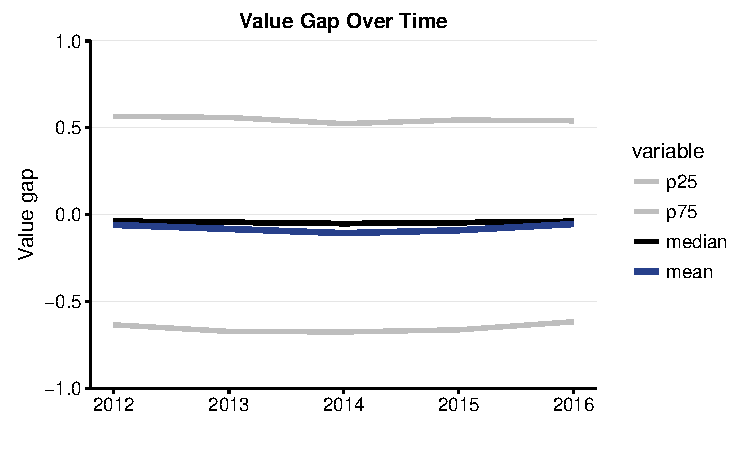
\includegraphics{Figs/value_time-1} \end{center}

\textbf{Trade gap across products}

\begin{Shaded}
\begin{Highlighting}[]
\CommentTok{#Across products?}
\NormalTok{products <-}\StringTok{ }\NormalTok{hs12[, .(}\DataTypeTok{mean =} \KeywordTok{as.double}\NormalTok{(}\KeywordTok{mean}\NormalTok{(Log_gap)),}
                     \DataTypeTok{median =} \KeywordTok{as.double}\NormalTok{(}\KeywordTok{median}\NormalTok{(Log_gap)),}
                     \DataTypeTok{p25 =} \KeywordTok{as.double}\NormalTok{(}\KeywordTok{quantile}\NormalTok{(Log_gap,.}\DecValTok{25}\NormalTok{)),}
                     \DataTypeTok{p75 =} \KeywordTok{as.double}\NormalTok{(}\KeywordTok{quantile}\NormalTok{(Log_gap,.}\DecValTok{75}\NormalTok{))}
\NormalTok{),}
\NormalTok{by=}\StringTok{ `}\DataTypeTok{Commodity Code}\StringTok{`}\NormalTok{]}

\KeywordTok{ggplot}\NormalTok{(}\DataTypeTok{data=}\NormalTok{products, }\KeywordTok{aes}\NormalTok{(mean)) +}
\StringTok{  }\KeywordTok{geom_histogram}\NormalTok{(}\DataTypeTok{col=}\StringTok{"royalblue4"}\NormalTok{,}
                 \DataTypeTok{fill=}\StringTok{"royalblue4"}\NormalTok{,}
                 \DataTypeTok{alpha=}\NormalTok{.}\DecValTok{2}\NormalTok{) +}
\StringTok{  }\KeywordTok{background_grid}\NormalTok{(}\DataTypeTok{major =} \StringTok{'y'}\NormalTok{, }\DataTypeTok{minor =} \StringTok{"none"}\NormalTok{) +}
\StringTok{  }\KeywordTok{scale_y_continuous}\NormalTok{(}\DataTypeTok{expand =} \KeywordTok{c}\NormalTok{(}\DecValTok{0}\NormalTok{, }\DecValTok{0}\NormalTok{), }\DataTypeTok{limits =} \KeywordTok{c}\NormalTok{(}\DecValTok{0}\NormalTok{,}\DecValTok{150}\NormalTok{), }\DataTypeTok{minor_breaks =} \OtherTok{NULL}\NormalTok{) +}
\StringTok{  }\KeywordTok{labs}\NormalTok{(}\DataTypeTok{title=}\StringTok{"Mean Trade Gap Across Products"}\NormalTok{) +}
\StringTok{  }\KeywordTok{labs}\NormalTok{(}\DataTypeTok{x=}\StringTok{"Trade gap"}\NormalTok{, }\DataTypeTok{y=}\StringTok{"Number of products"}\NormalTok{)}
\end{Highlighting}
\end{Shaded}

\begin{center}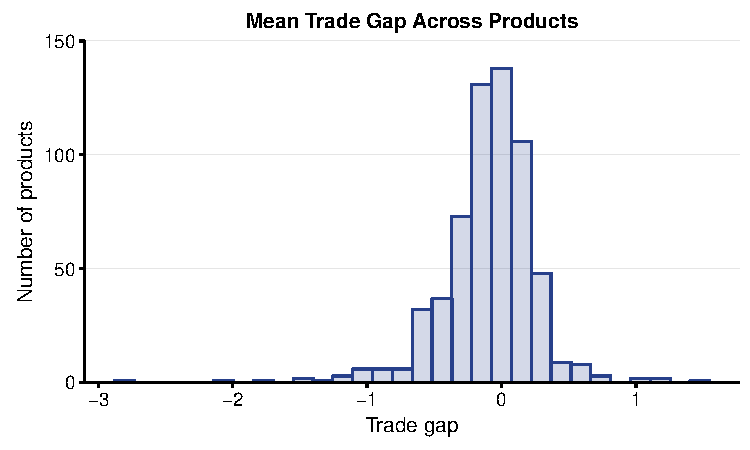
\includegraphics{Figs/value_products-1} \end{center}

\begin{Shaded}
\begin{Highlighting}[]
\KeywordTok{ggplot}\NormalTok{(}\DataTypeTok{data=}\NormalTok{products, }\KeywordTok{aes}\NormalTok{(median)) +}
\StringTok{  }\KeywordTok{geom_histogram}\NormalTok{(}\DataTypeTok{col=}\StringTok{"royalblue4"}\NormalTok{,}
                 \DataTypeTok{fill=}\StringTok{"royalblue4"}\NormalTok{,}
                 \DataTypeTok{alpha=}\NormalTok{.}\DecValTok{2}\NormalTok{) +}
\StringTok{  }\KeywordTok{background_grid}\NormalTok{(}\DataTypeTok{major =} \StringTok{'y'}\NormalTok{, }\DataTypeTok{minor =} \StringTok{"none"}\NormalTok{) +}
\StringTok{  }\KeywordTok{scale_y_continuous}\NormalTok{(}\DataTypeTok{expand =} \KeywordTok{c}\NormalTok{(}\DecValTok{0}\NormalTok{, }\DecValTok{0}\NormalTok{), }\DataTypeTok{limits =} \KeywordTok{c}\NormalTok{(}\DecValTok{0}\NormalTok{,}\DecValTok{350}\NormalTok{),  }\DataTypeTok{breaks=}\KeywordTok{seq}\NormalTok{(}\DecValTok{0}\NormalTok{, }\DecValTok{350}\NormalTok{, }\DecValTok{50}\NormalTok{)) +}
\StringTok{  }\KeywordTok{labs}\NormalTok{(}\DataTypeTok{title=}\StringTok{"Median Trade Gap Across Products"}\NormalTok{) +}
\StringTok{  }\KeywordTok{labs}\NormalTok{(}\DataTypeTok{x=}\StringTok{"Trade gap"}\NormalTok{, }\DataTypeTok{y=}\StringTok{"Number of products"}\NormalTok{)}
\end{Highlighting}
\end{Shaded}

\begin{center}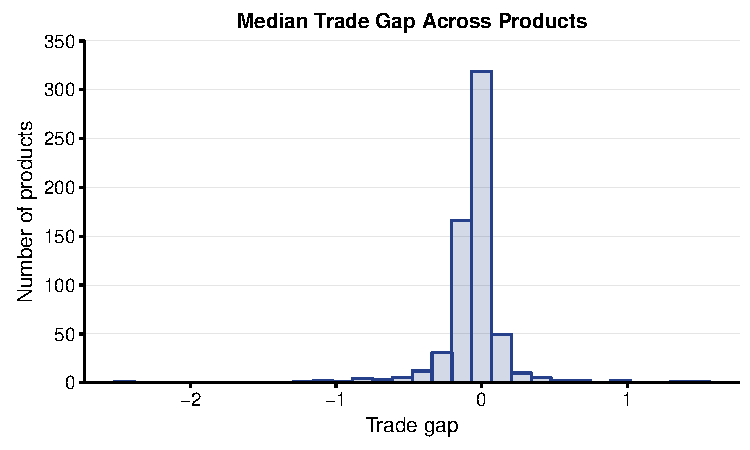
\includegraphics{Figs/value_products-2} \end{center}

\begin{Shaded}
\begin{Highlighting}[]
\KeywordTok{ggplot}\NormalTok{(}\DataTypeTok{data=}\NormalTok{products, }\KeywordTok{aes}\NormalTok{(p25)) +}
\StringTok{  }\KeywordTok{geom_histogram}\NormalTok{(}\DataTypeTok{col=}\StringTok{"royalblue4"}\NormalTok{,}
                 \DataTypeTok{fill=}\StringTok{"royalblue4"}\NormalTok{,}
                 \DataTypeTok{alpha=}\NormalTok{.}\DecValTok{2}\NormalTok{) +}
\StringTok{  }\KeywordTok{background_grid}\NormalTok{(}\DataTypeTok{major =} \StringTok{'y'}\NormalTok{, }\DataTypeTok{minor =} \StringTok{"none"}\NormalTok{) +}
\StringTok{  }\KeywordTok{scale_y_continuous}\NormalTok{(}\DataTypeTok{expand =} \KeywordTok{c}\NormalTok{(}\DecValTok{0}\NormalTok{, }\DecValTok{0}\NormalTok{),  }\DataTypeTok{limits =} \KeywordTok{c}\NormalTok{(}\DecValTok{0}\NormalTok{,}\DecValTok{150}\NormalTok{), }\DataTypeTok{minor_breaks =} \OtherTok{NULL}\NormalTok{) +}
\StringTok{  }\KeywordTok{labs}\NormalTok{(}\DataTypeTok{title=}\StringTok{"25th Percentile Trade Gap Across Products"}\NormalTok{) +}
\StringTok{  }\KeywordTok{labs}\NormalTok{(}\DataTypeTok{x=}\StringTok{"Trade gap"}\NormalTok{, }\DataTypeTok{y=}\StringTok{"Number of products"}\NormalTok{)}
\end{Highlighting}
\end{Shaded}

\begin{center}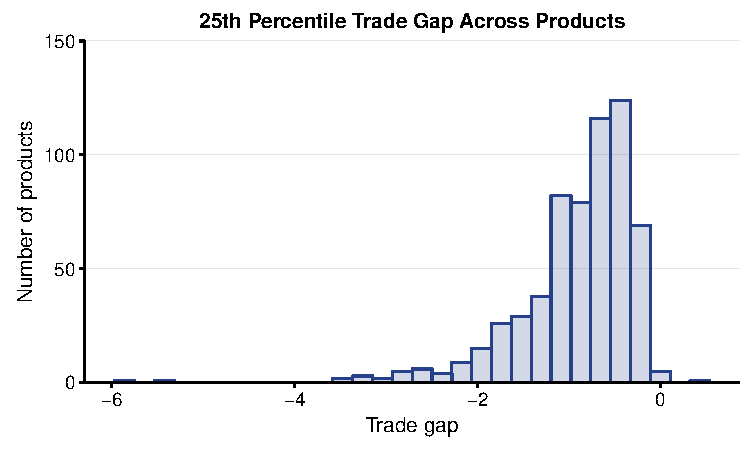
\includegraphics{Figs/value_products-3} \end{center}

\begin{Shaded}
\begin{Highlighting}[]
\KeywordTok{ggplot}\NormalTok{(}\DataTypeTok{data=}\NormalTok{products, }\KeywordTok{aes}\NormalTok{(p75)) +}
\StringTok{  }\KeywordTok{geom_histogram}\NormalTok{(}\DataTypeTok{col=}\StringTok{"royalblue4"}\NormalTok{,}
                 \DataTypeTok{fill=}\StringTok{"royalblue4"}\NormalTok{,}
                 \DataTypeTok{alpha=}\NormalTok{.}\DecValTok{2}\NormalTok{) +}
\StringTok{  }\KeywordTok{background_grid}\NormalTok{(}\DataTypeTok{major =} \StringTok{'y'}\NormalTok{, }\DataTypeTok{minor =} \StringTok{"none"}\NormalTok{) +}
\StringTok{  }\KeywordTok{scale_y_continuous}\NormalTok{(}\DataTypeTok{expand =} \KeywordTok{c}\NormalTok{(}\DecValTok{0}\NormalTok{, }\DecValTok{0}\NormalTok{),  }\DataTypeTok{limits =} \KeywordTok{c}\NormalTok{(}\DecValTok{0}\NormalTok{, }\DecValTok{150}\NormalTok{), }\DataTypeTok{minor_breaks =} \OtherTok{NULL}\NormalTok{) +}
\StringTok{  }\KeywordTok{labs}\NormalTok{(}\DataTypeTok{title=}\StringTok{"75th Percentile Trade Gap Across Products"}\NormalTok{) +}
\StringTok{  }\KeywordTok{labs}\NormalTok{(}\DataTypeTok{x=}\StringTok{"Trade gap"}\NormalTok{, }\DataTypeTok{y=}\StringTok{"Number of products"}\NormalTok{)}
\end{Highlighting}
\end{Shaded}

\begin{center}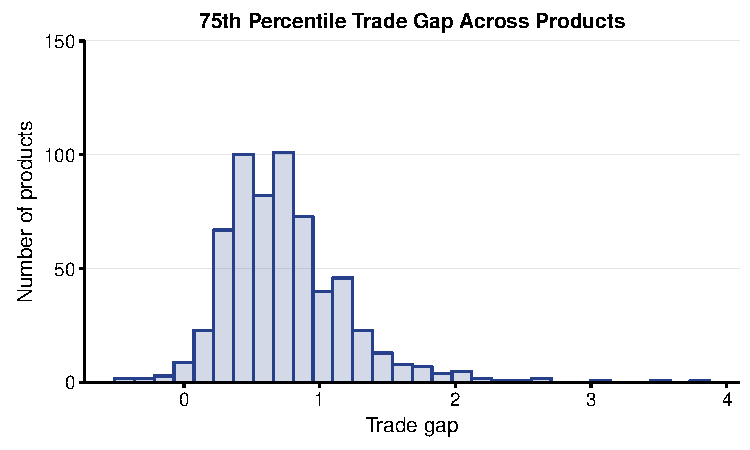
\includegraphics{Figs/value_products-4} \end{center}

\textbf{Trade gap across country pairs}

\begin{Shaded}
\begin{Highlighting}[]
\CommentTok{#Across countries?}
\NormalTok{countries <-}\StringTok{ }\NormalTok{hs12[, .(}\DataTypeTok{mean =} \KeywordTok{as.double}\NormalTok{(}\KeywordTok{mean}\NormalTok{(Log_gap)),}
                      \DataTypeTok{median =} \KeywordTok{as.double}\NormalTok{(}\KeywordTok{median}\NormalTok{(Log_gap)),}
                      \DataTypeTok{p25 =} \KeywordTok{as.double}\NormalTok{(}\KeywordTok{quantile}\NormalTok{(Log_gap,.}\DecValTok{25}\NormalTok{)),}
                      \DataTypeTok{p75 =} \KeywordTok{as.double}\NormalTok{(}\KeywordTok{quantile}\NormalTok{(Log_gap,.}\DecValTok{75}\NormalTok{))}
\NormalTok{),}
\NormalTok{by=}\StringTok{ }\KeywordTok{c}\NormalTok{(}\StringTok{"Importer"}\NormalTok{, }\StringTok{"Exporter"}\NormalTok{)]}

\KeywordTok{ggplot}\NormalTok{(}\DataTypeTok{data=}\NormalTok{countries, }\KeywordTok{aes}\NormalTok{(mean)) +}
\StringTok{  }\KeywordTok{geom_histogram}\NormalTok{(}\DataTypeTok{col=}\StringTok{"royalblue4"}\NormalTok{,}
                 \DataTypeTok{fill=}\StringTok{"royalblue4"}\NormalTok{,}
                 \DataTypeTok{alpha=}\NormalTok{.}\DecValTok{2}\NormalTok{) +}
\StringTok{  }\KeywordTok{background_grid}\NormalTok{(}\DataTypeTok{major =} \StringTok{'y'}\NormalTok{, }\DataTypeTok{minor =} \StringTok{"none"}\NormalTok{) +}
\StringTok{  }\KeywordTok{scale_y_continuous}\NormalTok{(}\DataTypeTok{expand =} \KeywordTok{c}\NormalTok{(}\DecValTok{0}\NormalTok{, }\DecValTok{0}\NormalTok{), }\DataTypeTok{limits =} \KeywordTok{c}\NormalTok{(}\DecValTok{0}\NormalTok{, }\DecValTok{1500}\NormalTok{),  }\DataTypeTok{minor_breaks =} \OtherTok{NULL}\NormalTok{) +}
\StringTok{  }\KeywordTok{labs}\NormalTok{(}\DataTypeTok{title=}\StringTok{"Mean Trade Gap Across Country Pairs"}\NormalTok{) +}
\StringTok{  }\KeywordTok{labs}\NormalTok{(}\DataTypeTok{x=}\StringTok{"Trade gap"}\NormalTok{, }\DataTypeTok{y=}\StringTok{"Number of pairs"}\NormalTok{)}
\end{Highlighting}
\end{Shaded}

\begin{center}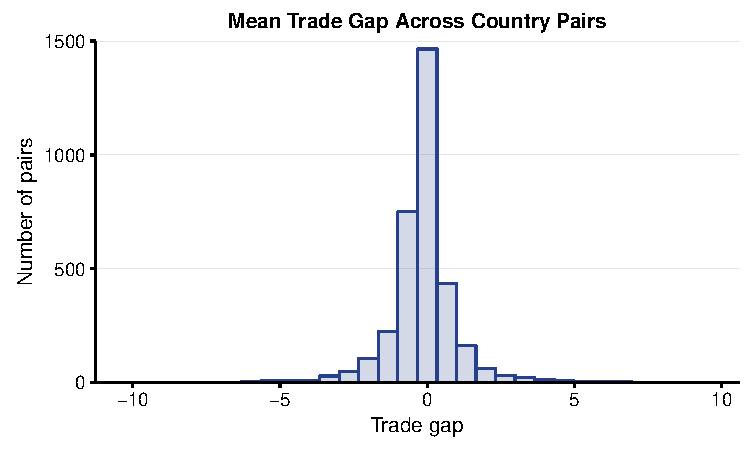
\includegraphics{Figs/value_pairs-1} \end{center}

\begin{Shaded}
\begin{Highlighting}[]
\KeywordTok{ggplot}\NormalTok{(}\DataTypeTok{data=}\NormalTok{countries, }\KeywordTok{aes}\NormalTok{(median)) +}
\StringTok{  }\KeywordTok{geom_histogram}\NormalTok{(}\DataTypeTok{col=}\StringTok{"royalblue4"}\NormalTok{,}
                 \DataTypeTok{fill=}\StringTok{"royalblue4"}\NormalTok{,}
                 \DataTypeTok{alpha=}\NormalTok{.}\DecValTok{2}\NormalTok{) +}
\StringTok{  }\KeywordTok{background_grid}\NormalTok{(}\DataTypeTok{major =} \StringTok{'y'}\NormalTok{, }\DataTypeTok{minor =} \StringTok{"none"}\NormalTok{) +}
\StringTok{  }\KeywordTok{scale_y_continuous}\NormalTok{(}\DataTypeTok{expand =} \KeywordTok{c}\NormalTok{(}\DecValTok{0}\NormalTok{, }\DecValTok{0}\NormalTok{), }\DataTypeTok{limits =} \KeywordTok{c}\NormalTok{(}\DecValTok{0}\NormalTok{, }\DecValTok{2000}\NormalTok{),  }\DataTypeTok{minor_breaks =} \OtherTok{NULL}\NormalTok{) +}
\StringTok{  }\KeywordTok{labs}\NormalTok{(}\DataTypeTok{title=}\StringTok{"Median Trade Gap Across Country Pairs"}\NormalTok{) +}
\StringTok{  }\KeywordTok{labs}\NormalTok{(}\DataTypeTok{x=}\StringTok{"Trade gap"}\NormalTok{, }\DataTypeTok{y=}\StringTok{"Number of pairs"}\NormalTok{)}
\end{Highlighting}
\end{Shaded}

\begin{center}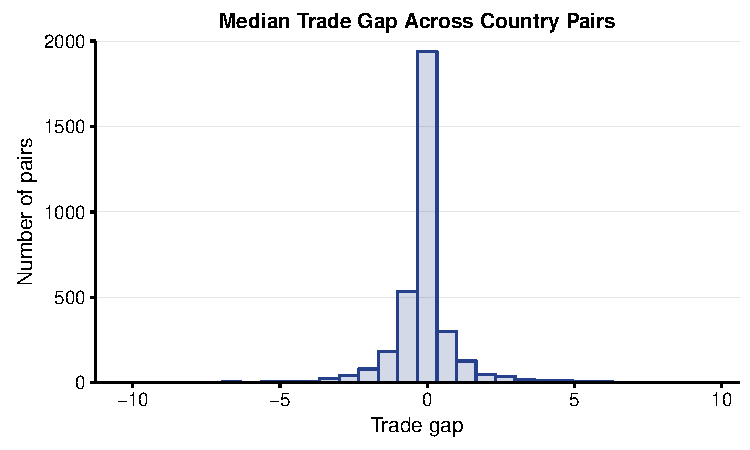
\includegraphics{Figs/value_pairs-2} \end{center}

\begin{Shaded}
\begin{Highlighting}[]
\KeywordTok{ggplot}\NormalTok{(}\DataTypeTok{data=}\NormalTok{countries, }\KeywordTok{aes}\NormalTok{(p25)) +}
\StringTok{  }\KeywordTok{geom_histogram}\NormalTok{(}\DataTypeTok{col=}\StringTok{"royalblue4"}\NormalTok{,}
                 \DataTypeTok{fill=}\StringTok{"royalblue4"}\NormalTok{,}
                 \DataTypeTok{alpha=}\NormalTok{.}\DecValTok{2}\NormalTok{) +}
\StringTok{  }\KeywordTok{background_grid}\NormalTok{(}\DataTypeTok{major =} \StringTok{'y'}\NormalTok{, }\DataTypeTok{minor =} \StringTok{"none"}\NormalTok{) +}
\StringTok{  }\KeywordTok{scale_y_continuous}\NormalTok{(}\DataTypeTok{expand =} \KeywordTok{c}\NormalTok{(}\DecValTok{0}\NormalTok{, }\DecValTok{0}\NormalTok{), }\DataTypeTok{limits =} \KeywordTok{c}\NormalTok{(}\DecValTok{0}\NormalTok{, }\DecValTok{1500}\NormalTok{),  }\DataTypeTok{minor_breaks =} \OtherTok{NULL}\NormalTok{) +}
\StringTok{  }\KeywordTok{labs}\NormalTok{(}\DataTypeTok{title=}\StringTok{"25th Percentile Trade Gap Across Country Pairs"}\NormalTok{) +}
\StringTok{  }\KeywordTok{labs}\NormalTok{(}\DataTypeTok{x=}\StringTok{"Trade gap"}\NormalTok{, }\DataTypeTok{y=}\StringTok{"Number of pairs"}\NormalTok{)}
\end{Highlighting}
\end{Shaded}

\begin{center}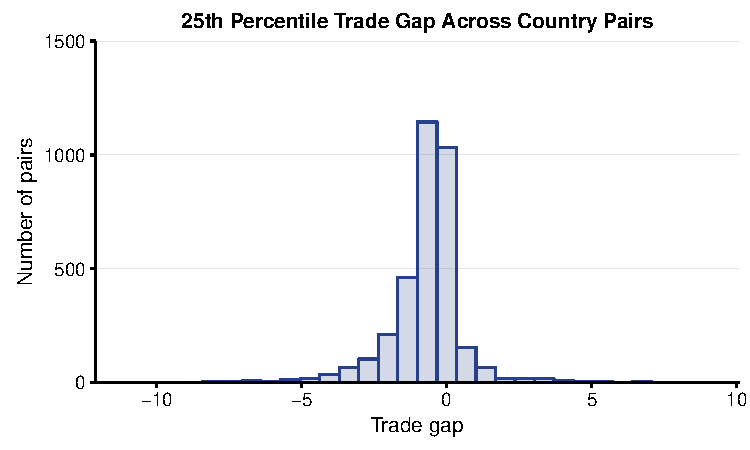
\includegraphics{Figs/value_pairs-3} \end{center}

\begin{Shaded}
\begin{Highlighting}[]
\KeywordTok{ggplot}\NormalTok{(}\DataTypeTok{data=}\NormalTok{countries, }\KeywordTok{aes}\NormalTok{(p75)) +}
\StringTok{  }\KeywordTok{geom_histogram}\NormalTok{(}\DataTypeTok{col=}\StringTok{"royalblue4"}\NormalTok{,}
                 \DataTypeTok{fill=}\StringTok{"royalblue4"}\NormalTok{,}
                 \DataTypeTok{alpha=}\NormalTok{.}\DecValTok{2}\NormalTok{) +}
\StringTok{  }\KeywordTok{background_grid}\NormalTok{(}\DataTypeTok{major =} \StringTok{'y'}\NormalTok{, }\DataTypeTok{minor =} \StringTok{"none"}\NormalTok{) +}
\StringTok{  }\KeywordTok{scale_y_continuous}\NormalTok{(}\DataTypeTok{expand =} \KeywordTok{c}\NormalTok{(}\DecValTok{0}\NormalTok{, }\DecValTok{0}\NormalTok{), }\DataTypeTok{limits =} \KeywordTok{c}\NormalTok{(}\DecValTok{0}\NormalTok{, }\DecValTok{2000}\NormalTok{),  }\DataTypeTok{minor_breaks =} \OtherTok{NULL}\NormalTok{) +}
\StringTok{  }\KeywordTok{labs}\NormalTok{(}\DataTypeTok{title=}\StringTok{"75th Percentile Trade Gap Across Country Pairs"}\NormalTok{) +}
\StringTok{  }\KeywordTok{labs}\NormalTok{(}\DataTypeTok{x=}\StringTok{"Trade gap"}\NormalTok{, }\DataTypeTok{y=}\StringTok{"Number of pairs"}\NormalTok{)}
\end{Highlighting}
\end{Shaded}

\begin{center}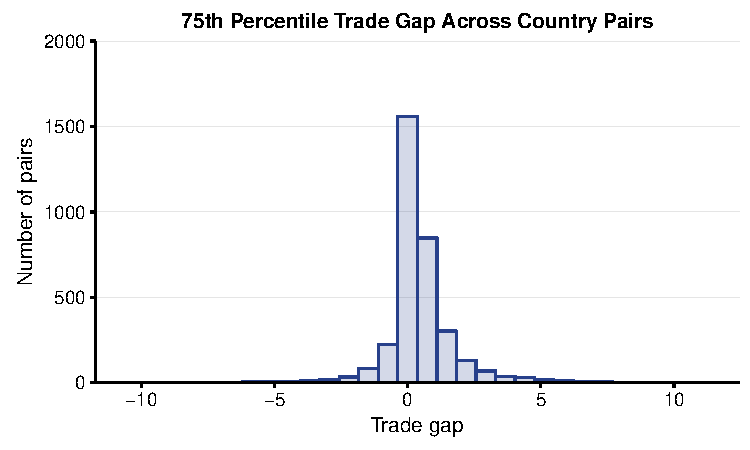
\includegraphics{Figs/value_pairs-4} \end{center}

\begin{Shaded}
\begin{Highlighting}[]
\KeywordTok{rm}\NormalTok{(periods, products, countries)}
\end{Highlighting}
\end{Shaded}

\textbf{Year coefficients controlling for product codes and country
pairs}

\begin{Shaded}
\begin{Highlighting}[]
\NormalTok{hs12$Period <-}\StringTok{ }\KeywordTok{as.Date}\NormalTok{(hs12$Period, }\StringTok{"%Y"}\NormalTok{)}
\NormalTok{hs12$Period <-}\StringTok{ }\KeywordTok{floor_date}\NormalTok{(hs12$Period,}\StringTok{"year"}\NormalTok{)}

\NormalTok{hs12$Period.f <-}\StringTok{ }\KeywordTok{factor}\NormalTok{(hs12$Period)}
\NormalTok{hs12$Products.f <-}\StringTok{ }\KeywordTok{factor}\NormalTok{(hs12$}\StringTok{`}\DataTypeTok{Commodity Code}\StringTok{`}\NormalTok{)}

\NormalTok{hs12$Importer.f <-}\StringTok{ }\KeywordTok{factor}\NormalTok{(hs12$}\StringTok{`}\DataTypeTok{Reporter Code}\StringTok{`}\NormalTok{)}
\NormalTok{hs12$Exporter.f <-}\StringTok{ }\KeywordTok{factor}\NormalTok{(hs12$}\StringTok{`}\DataTypeTok{Partner Code}\StringTok{`}\NormalTok{)}
\NormalTok{hs12$Pairs.f <-}\StringTok{ }\KeywordTok{with}\NormalTok{(hs12, }\KeywordTok{interaction}\NormalTok{(Importer.f, Exporter.f))}

\NormalTok{reg <-}\StringTok{ }\KeywordTok{felm}\NormalTok{(Log_gap ~}\StringTok{ }\DecValTok{1} \NormalTok{|}\StringTok{ }\NormalTok{Period.f +}\StringTok{ }\NormalTok{Products.f +}\StringTok{ }\NormalTok{Pairs.f,}
            \DataTypeTok{data =} \NormalTok{hs12,}
            \DataTypeTok{exactDOF =} \OtherTok{FALSE}\NormalTok{,}
            \DataTypeTok{keepX =} \OtherTok{FALSE}\NormalTok{,}
            \DataTypeTok{keepCX =} \OtherTok{FALSE}\NormalTok{)}

\NormalTok{fes <-}\StringTok{ }\KeywordTok{getfe}\NormalTok{(reg,}
             \DataTypeTok{se=}\OtherTok{TRUE}\NormalTok{,}
             \DataTypeTok{bN =} \DecValTok{50}
\NormalTok{)}

\NormalTok{periodfes <-}\StringTok{ }\KeywordTok{subset}\NormalTok{(fes,fe ==}\StringTok{ "Period.f"}\NormalTok{)}

\NormalTok{periodfes$ci_ub <-}\StringTok{ }\NormalTok{periodfes$effect +}\StringTok{ }\NormalTok{(}\FloatTok{1.96} \NormalTok{*}\StringTok{ }\NormalTok{periodfes$se)}
\NormalTok{periodfes$ci_lb <-}\StringTok{ }\NormalTok{periodfes$effect -}\StringTok{ }\NormalTok{(}\FloatTok{1.96} \NormalTok{*}\StringTok{ }\NormalTok{periodfes$se)}
\NormalTok{periodfes <-}\StringTok{ }\KeywordTok{merge}\NormalTok{(periodfes,}\KeywordTok{unique}\NormalTok{(hs12[,}\KeywordTok{list}\NormalTok{(Period,Period.f)]),}\DataTypeTok{by.x =} \StringTok{"idx"}\NormalTok{,}\DataTypeTok{by.y=}\StringTok{"Period.f"}\NormalTok{)}
\NormalTok{periodfes <-}\StringTok{ }\KeywordTok{rename}\NormalTok{(periodfes, }\DataTypeTok{period =} \NormalTok{Period)}

\KeywordTok{ggplot}\NormalTok{(}\DataTypeTok{data =} \NormalTok{periodfes, }\KeywordTok{aes}\NormalTok{(period,effect)) +}
\StringTok{  }\KeywordTok{geom_errorbar}\NormalTok{(}\KeywordTok{aes}\NormalTok{(}\DataTypeTok{ymin =} \NormalTok{ci_lb, }\DataTypeTok{ymax =} \NormalTok{ci_ub), }\DataTypeTok{color =} \StringTok{"grey35"}\NormalTok{) +}
\StringTok{  }\KeywordTok{geom_line}\NormalTok{(}\DataTypeTok{color =} \StringTok{"royalblue4"}\NormalTok{, }\DataTypeTok{size =} \DecValTok{1}\NormalTok{) +}
\StringTok{  }\KeywordTok{geom_point}\NormalTok{(}\DataTypeTok{color =} \StringTok{"royalblue4"}\NormalTok{) +}
\StringTok{  }\KeywordTok{background_grid}\NormalTok{(}\DataTypeTok{major =} \StringTok{'y'}\NormalTok{, }\DataTypeTok{minor =} \StringTok{"none"}\NormalTok{) +}
\StringTok{  }\KeywordTok{scale_y_continuous}\NormalTok{(}\DataTypeTok{expand =} \KeywordTok{c}\NormalTok{(}\DecValTok{0}\NormalTok{, }\DecValTok{0}\NormalTok{), }\DataTypeTok{limits =} \KeywordTok{c}\NormalTok{(-.}\DecValTok{050}\NormalTok{,.}\DecValTok{075}\NormalTok{), }\DataTypeTok{minor_breaks =} \OtherTok{NULL}\NormalTok{) +}
\StringTok{  }\KeywordTok{xlab}\NormalTok{(}\DataTypeTok{label =} \StringTok{""}\NormalTok{) +}
\StringTok{  }\KeywordTok{ylab}\NormalTok{(}\DataTypeTok{label =} \StringTok{"Trade gap"}\NormalTok{) +}
\StringTok{  }\KeywordTok{labs}\NormalTok{(}\DataTypeTok{title =} \StringTok{"Trade Gap Over Time, Controlling for Product/Country Pair"}\NormalTok{)}
\end{Highlighting}
\end{Shaded}

\begin{center}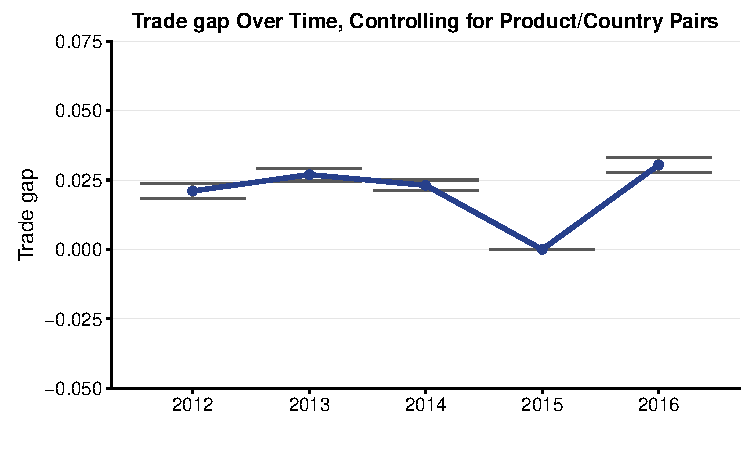
\includegraphics{Figs/value_years_reg-1} \end{center}

Why the 2016 bump? Could it be something to do with how they revise
value estimates when they get more data or convert to most recent HS
classification?

\textbf{Product code coefficients controlling for country pairs and
years}

\begin{Shaded}
\begin{Highlighting}[]
\NormalTok{productfes <-}\StringTok{ }\KeywordTok{subset}\NormalTok{(fes,fe ==}\StringTok{ "Products.f"}\NormalTok{)}
\NormalTok{productfes <-}\StringTok{ }\NormalTok{productfes[,}\KeywordTok{c}\NormalTok{(}\StringTok{"effect"}\NormalTok{,}\StringTok{"idx"}\NormalTok{)]}

\KeywordTok{ggplot}\NormalTok{(}\DataTypeTok{data=}\NormalTok{productfes, }\KeywordTok{aes}\NormalTok{(effect)) +}
\StringTok{  }\KeywordTok{geom_histogram}\NormalTok{(}\DataTypeTok{col=}\StringTok{"royalblue4"}\NormalTok{,}
                 \DataTypeTok{fill=}\StringTok{"royalblue4"}\NormalTok{,}
                 \DataTypeTok{alpha=}\NormalTok{.}\DecValTok{2}\NormalTok{) +}
\StringTok{  }\KeywordTok{background_grid}\NormalTok{(}\DataTypeTok{major =} \StringTok{'y'}\NormalTok{, }\DataTypeTok{minor =} \StringTok{"none"}\NormalTok{) +}
\StringTok{  }\KeywordTok{scale_y_continuous}\NormalTok{(}\DataTypeTok{expand =} \KeywordTok{c}\NormalTok{(}\DecValTok{0}\NormalTok{, }\DecValTok{0}\NormalTok{), }\DataTypeTok{limits =} \KeywordTok{c}\NormalTok{(}\DecValTok{0}\NormalTok{,}\DecValTok{150}\NormalTok{), }\DataTypeTok{minor_breaks =} \OtherTok{NULL}\NormalTok{) +}
\StringTok{  }\KeywordTok{labs}\NormalTok{(}\DataTypeTok{title=}\StringTok{"Trade Gap Across Products, Controlling for Country Pair/Year"}\NormalTok{) +}
\StringTok{  }\KeywordTok{labs}\NormalTok{(}\DataTypeTok{x=}\StringTok{"Trade gap"}\NormalTok{, }\DataTypeTok{y=}\StringTok{"Number of products"}\NormalTok{)}
\end{Highlighting}
\end{Shaded}

\begin{center}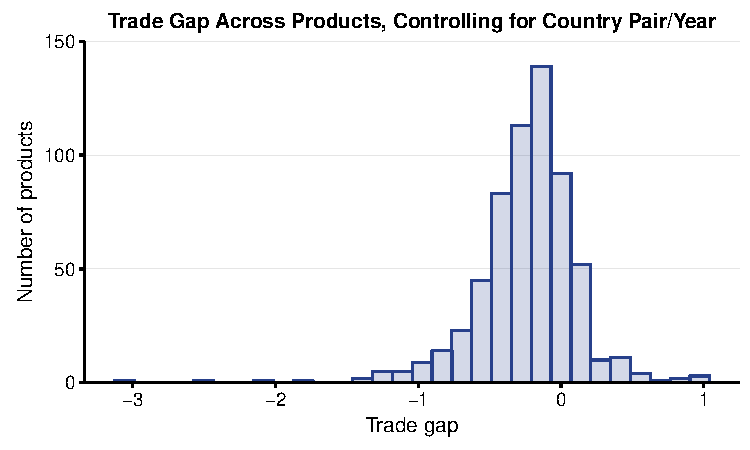
\includegraphics{Figs/value_products_reg-1} \end{center}

\textbf{Country pair coefficients controlling for years and product
codes}

\begin{Shaded}
\begin{Highlighting}[]
\NormalTok{pairfes <-}\StringTok{ }\KeywordTok{subset}\NormalTok{(fes,fe ==}\StringTok{ "Pairs.f"}\NormalTok{)}
\NormalTok{pairfes <-}\StringTok{ }\NormalTok{pairfes[,}\KeywordTok{c}\NormalTok{(}\StringTok{"effect"}\NormalTok{,}\StringTok{"idx"}\NormalTok{)]}

\KeywordTok{ggplot}\NormalTok{(}\DataTypeTok{data=}\NormalTok{pairfes, }\KeywordTok{aes}\NormalTok{(effect)) +}
\StringTok{  }\KeywordTok{geom_histogram}\NormalTok{(}\DataTypeTok{col=}\StringTok{"royalblue4"}\NormalTok{,}
                 \DataTypeTok{fill=}\StringTok{"royalblue4"}\NormalTok{,}
                 \DataTypeTok{alpha=}\NormalTok{.}\DecValTok{2}\NormalTok{) +}
\StringTok{  }\KeywordTok{background_grid}\NormalTok{(}\DataTypeTok{major =} \StringTok{'y'}\NormalTok{, }\DataTypeTok{minor =} \StringTok{"none"}\NormalTok{) +}
\StringTok{  }\KeywordTok{scale_y_continuous}\NormalTok{(}\DataTypeTok{expand =} \KeywordTok{c}\NormalTok{(}\DecValTok{0}\NormalTok{, }\DecValTok{0}\NormalTok{), }\DataTypeTok{limits =} \KeywordTok{c}\NormalTok{(}\DecValTok{0}\NormalTok{,}\DecValTok{1500}\NormalTok{), }\DataTypeTok{minor_breaks =} \OtherTok{NULL}\NormalTok{) +}
\StringTok{  }\KeywordTok{labs}\NormalTok{(}\DataTypeTok{title=}\StringTok{"Trade Gap Across Country Pairs, Controlling for Product/Year"}\NormalTok{) +}
\StringTok{  }\KeywordTok{labs}\NormalTok{(}\DataTypeTok{x=}\StringTok{"Trade gap"}\NormalTok{, }\DataTypeTok{y=}\StringTok{"Number of country pairs"}\NormalTok{)}
\end{Highlighting}
\end{Shaded}

\begin{center}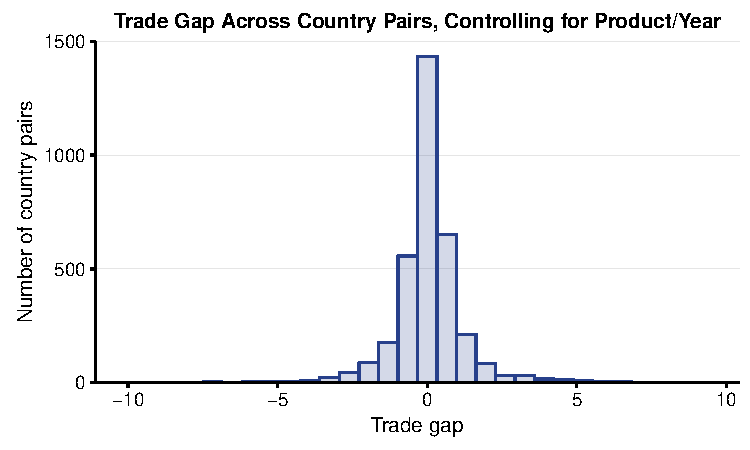
\includegraphics{Figs/value_pairs_reg-1} \end{center}

\begin{Shaded}
\begin{Highlighting}[]
\KeywordTok{rm}\NormalTok{(fes, hs12, pairfes, periodfes, productfes, reg)}
\end{Highlighting}
\end{Shaded}

\section{Quantity Trade Gap}\label{quantity-trade-gap}

The difference between what the exporting country reports and what the
importing country reports in netweight (kg).

\textbf{Coverage}

\begin{Shaded}
\begin{Highlighting}[]
\KeywordTok{options}\NormalTok{(}\DataTypeTok{digits=}\DecValTok{2}\NormalTok{)}

\KeywordTok{load}\NormalTok{(}\KeywordTok{paste}\NormalTok{(DataPath,}\StringTok{"Analysis Data/hs12.Rda"}\NormalTok{, }\DataTypeTok{sep =} \StringTok{"/"}\NormalTok{))}
\NormalTok{hs12 <-}\StringTok{ }\KeywordTok{as.data.table}\NormalTok{(hs12)}

\CommentTok{#Remove observations where one or more countries do not report quantities. 748,839 rows deleted. }
\NormalTok{hs12 <-}\StringTok{ }\NormalTok{hs12[!}\KeywordTok{is.na}\NormalTok{(Qty_log_gap)]}

\CommentTok{#There are 411 instances where `qty_log_gap` = inf. }
\CommentTok{#I removed them -- something else we should do?}
\NormalTok{hs12 <-}\StringTok{ }\NormalTok{hs12[!}\KeywordTok{is.infinite}\NormalTok{(Qty_log_gap)]}

\CommentTok{#For each year, how many product*country pairs / all possible product*country pairs?}

\NormalTok{product <-}\StringTok{ }\NormalTok{hs12[, }\KeywordTok{uniqueN}\NormalTok{(}\StringTok{`}\DataTypeTok{Commodity Code}\StringTok{`}\NormalTok{)]}
\NormalTok{product_year <-}\StringTok{ }\NormalTok{hs12[, }\KeywordTok{uniqueN}\NormalTok{(}\StringTok{`}\DataTypeTok{Commodity Code}\StringTok{`}\NormalTok{), by=Period]}
\NormalTok{product_year <-}\StringTok{ }\KeywordTok{rename}\NormalTok{(product_year, }\DataTypeTok{Products =} \NormalTok{V1)}

\NormalTok{pair <-}\StringTok{ }\KeywordTok{unique}\NormalTok{(}\KeywordTok{setDT}\NormalTok{(hs12), }\DataTypeTok{by =} \KeywordTok{c}\NormalTok{(}\StringTok{"Importer"}\NormalTok{, }\StringTok{"Exporter"}\NormalTok{))}
\NormalTok{pair <-}\StringTok{ }\NormalTok{pair[, .N]}
\NormalTok{pair_year <-}\StringTok{ }\KeywordTok{unique}\NormalTok{(}\KeywordTok{setDT}\NormalTok{(hs12), }\DataTypeTok{by =} \KeywordTok{c}\NormalTok{(}\StringTok{"Importer"}\NormalTok{, }\StringTok{"Exporter"}\NormalTok{, }\StringTok{"Period"}\NormalTok{))}
\NormalTok{pair_year <-}\StringTok{ }\NormalTok{pair_year[, .N, by=Period]}
\NormalTok{pair_year <-}\StringTok{ }\KeywordTok{rename}\NormalTok{(pair_year, }\DataTypeTok{Pairs =} \NormalTok{N)}

\NormalTok{year_coverage <-}\StringTok{ }\KeywordTok{merge}\NormalTok{(product_year, pair_year)}
\NormalTok{year_coverage$Total_products <-}\StringTok{ }\NormalTok{product}
\NormalTok{year_coverage$Total_pairs <-}\StringTok{ }\NormalTok{pair}

\NormalTok{year_coverage$Coverage <-}\StringTok{ }\NormalTok{(year_coverage$Products*year_coverage$Pairs)/}
\StringTok{  }\NormalTok{(year_coverage$Total_products*year_coverage$Total_pair)}

\NormalTok{year_coverage}
\end{Highlighting}
\end{Shaded}

\begin{verbatim}
##    Period Products Pairs Total_products Total_pairs Coverage
## 1:   2012      604  1652            608        3292     0.50
## 2:   2013      604  2153            608        3292     0.65
## 3:   2014      603  2441            608        3292     0.74
## 4:   2015      601  2519            608        3292     0.76
## 5:   2016      605  1778            608        3292     0.54
\end{verbatim}

\begin{Shaded}
\begin{Highlighting}[]
\KeywordTok{rm}\NormalTok{(pair_year, product_year, year_coverage)}

\CommentTok{#For each product, how many year*country pairs / all possible year*country pairs?}

\NormalTok{year <-}\StringTok{ }\NormalTok{hs12[, }\KeywordTok{uniqueN}\NormalTok{(}\StringTok{`}\DataTypeTok{Period}\StringTok{`}\NormalTok{)]}
\NormalTok{year_product <-}\StringTok{ }\NormalTok{hs12[, }\KeywordTok{uniqueN}\NormalTok{(}\StringTok{`}\DataTypeTok{Period}\StringTok{`}\NormalTok{), by=}\StringTok{`}\DataTypeTok{Commodity Code}\StringTok{`}\NormalTok{]}
\NormalTok{year_product <-}\StringTok{ }\KeywordTok{rename}\NormalTok{(year_product, }\DataTypeTok{Years =} \NormalTok{V1)}

\NormalTok{pair_product <-}\StringTok{ }\KeywordTok{unique}\NormalTok{(}\KeywordTok{setDT}\NormalTok{(hs12), }\DataTypeTok{by =} \KeywordTok{c}\NormalTok{(}\StringTok{"Importer"}\NormalTok{, }\StringTok{"Exporter"}\NormalTok{, }\StringTok{"Commodity Code"}\NormalTok{))}
\NormalTok{pair_product <-}\StringTok{ }\NormalTok{pair_product[, .N, by=}\StringTok{ }\NormalTok{.(}\StringTok{`}\DataTypeTok{Commodity Code}\StringTok{`}\NormalTok{)]}
\NormalTok{pair_product <-}\StringTok{ }\KeywordTok{rename}\NormalTok{(pair_product, }\DataTypeTok{Pairs =} \NormalTok{N)}

\NormalTok{product_coverage <-}\StringTok{ }\KeywordTok{merge}\NormalTok{(year_product, pair_product)}
\NormalTok{product_coverage$Total_years <-}\StringTok{ }\NormalTok{year}
\NormalTok{product_coverage$Total_pairs <-}\StringTok{ }\NormalTok{pair}

\NormalTok{product_coverage$Coverage <-}\StringTok{ }\NormalTok{(product_coverage$Years*product_coverage$Pairs)/}
\StringTok{  }\NormalTok{(product_coverage$Total_years*product_coverage$Total_pairs)}

\CommentTok{#Note: Quantity is not reported at the two-digit level}
\NormalTok{product_coverage[}\KeywordTok{order}\NormalTok{(Coverage)][}\DecValTok{1}\NormalTok{:}\DecValTok{10}\NormalTok{]}
\end{Highlighting}
\end{Shaded}

\begin{verbatim}
##     Commodity Code Years Pairs Total_years Total_pairs Coverage
##  1:         010612     1     2           5        3292  0.00012
##  2:         010231     2     2           5        3292  0.00024
##  3:         010633     2     2           5        3292  0.00024
##  4:         030356     2     2           5        3292  0.00024
##  5:         010239     3     3           5        3292  0.00055
##  6:         020830     4     3           5        3292  0.00073
##  7:         030446     3     4           5        3292  0.00073
##  8:         030455     3     4           5        3292  0.00073
##  9:         010613     4     5           5        3292  0.00122
## 10:         030564     4     5           5        3292  0.00122
\end{verbatim}

\begin{Shaded}
\begin{Highlighting}[]
\NormalTok{product_coverage[}\KeywordTok{order}\NormalTok{(-Coverage)][}\DecValTok{1}\NormalTok{:}\DecValTok{10}\NormalTok{]}
\end{Highlighting}
\end{Shaded}

\begin{verbatim}
##     Commodity Code Years Pairs Total_years Total_pairs Coverage
##  1:           0901     5  1231           5        3292     0.37
##  2:           0902     5  1022           5        3292     0.31
##  3:           0713     5   986           5        3292     0.30
##  4:           0910     5   982           5        3292     0.30
##  5:           0303     5   981           5        3292     0.30
##  6:           0406     5   940           5        3292     0.29
##  7:           0602     5   863           5        3292     0.26
##  8:           0904     5   863           5        3292     0.26
##  9:           0712     5   853           5        3292     0.26
## 10:           0402     5   847           5        3292     0.26
\end{verbatim}

\begin{Shaded}
\begin{Highlighting}[]
\KeywordTok{rm}\NormalTok{(year_product, pair_product, product_coverage)}

\CommentTok{#For each country pair, how many year*product / all possible year*product?}

\NormalTok{product_pair <-}\StringTok{ }\NormalTok{hs12[, }\KeywordTok{uniqueN}\NormalTok{(}\StringTok{`}\DataTypeTok{Commodity Code}\StringTok{`}\NormalTok{), by =}\StringTok{ }\KeywordTok{c}\NormalTok{(}\StringTok{"Importer"}\NormalTok{, }\StringTok{"Exporter"}\NormalTok{)]}
\NormalTok{product_pair <-}\StringTok{ }\KeywordTok{rename}\NormalTok{(product_pair, }\DataTypeTok{Products =} \NormalTok{V1)}

\NormalTok{year_pair <-}\StringTok{ }\NormalTok{hs12[, }\KeywordTok{uniqueN}\NormalTok{(}\StringTok{`}\DataTypeTok{Period}\StringTok{`}\NormalTok{), by =}\StringTok{ }\KeywordTok{c}\NormalTok{(}\StringTok{"Importer"}\NormalTok{, }\StringTok{"Exporter"}\NormalTok{)]}
\NormalTok{year_pair <-}\StringTok{ }\KeywordTok{rename}\NormalTok{(year_pair, }\DataTypeTok{Years =} \NormalTok{V1)}

\NormalTok{pair_coverage <-}\StringTok{ }\KeywordTok{merge}\NormalTok{(product_pair, year_pair, }\DataTypeTok{by =} \KeywordTok{c}\NormalTok{(}\StringTok{"Importer"}\NormalTok{, }\StringTok{"Exporter"}\NormalTok{))}
\NormalTok{pair_coverage$T_products <-}\StringTok{ }\NormalTok{product}
\NormalTok{pair_coverage$T_years <-}\StringTok{ }\NormalTok{year}

\NormalTok{pair_coverage$Coverage <-}\StringTok{ }\NormalTok{(pair_coverage$Products*pair_coverage$Years)/}
\StringTok{  }\NormalTok{(pair_coverage$T_products*pair_coverage$T_years)}

\NormalTok{pair_coverage$Exporter <-}\StringTok{ }\KeywordTok{strtrim}\NormalTok{(pair_coverage$Exporter, }\DecValTok{15}\NormalTok{)}
\NormalTok{pair_coverage[}\KeywordTok{order}\NormalTok{(Coverage)][}\DecValTok{1}\NormalTok{:}\DecValTok{10}\NormalTok{]}
\end{Highlighting}
\end{Shaded}

\begin{verbatim}
##      Importer   Exporter Products Years T_products T_years Coverage
##  1:   Albania Madagascar        1     1        608       5  0.00033
##  2:   Algeria Cabo Verde        1     1        608       5  0.00033
##  3:   Algeria     Guinea        1     1        608       5  0.00033
##  4:    Angola Costa Rica        1     1        608       5  0.00033
##  5:    Angola   Honduras        1     1        608       5  0.00033
##  6: Argentina    Hungary        1     1        608       5  0.00033
##  7: Argentina    Lebanon        1     1        608       5  0.00033
##  8:   Armenia     Cyprus        1     1        608       5  0.00033
##  9:   Armenia    Estonia        1     1        608       5  0.00033
## 10:   Austria   Cambodia        1     1        608       5  0.00033
\end{verbatim}

\begin{Shaded}
\begin{Highlighting}[]
\NormalTok{pair_coverage[}\KeywordTok{order}\NormalTok{(-Coverage)][}\DecValTok{1}\NormalTok{:}\DecValTok{10}\NormalTok{]}
\end{Highlighting}
\end{Shaded}

\begin{verbatim}
##       Importer Exporter Products Years T_products T_years Coverage
##  1:    Belgium   France      564     5        608       5     0.93
##  2:      Italy   France      542     5        608       5     0.89
##  3:    Germany   France      537     5        608       5     0.88
##  4: Luxembourg   France      536     5        608       5     0.88
##  5:     France  Belgium      526     5        608       5     0.87
##  6:     France    Italy      525     5        608       5     0.86
##  7: Luxembourg  Belgium      523     5        608       5     0.86
##  8:     France  Germany      519     5        608       5     0.85
##  9:      Italy  Germany      507     5        608       5     0.83
## 10:    Germany    Italy      505     5        608       5     0.83
\end{verbatim}

\begin{Shaded}
\begin{Highlighting}[]
\KeywordTok{rm}\NormalTok{(product_pair, year_pair, pair_coverage, pair, product, year)}
\end{Highlighting}
\end{Shaded}

\textbf{Quantity trade gap over time}

\begin{Shaded}
\begin{Highlighting}[]
\NormalTok{hs12$Period <-}\StringTok{ }\KeywordTok{as.Date}\NormalTok{(hs12$Period, }\StringTok{"%Y"}\NormalTok{)}
\NormalTok{hs12$Period <-}\StringTok{ }\KeywordTok{floor_date}\NormalTok{(hs12$Period,}\StringTok{"year"}\NormalTok{)}


\NormalTok{periods <-}\StringTok{ }\NormalTok{hs12[, .(}\DataTypeTok{mean =} \KeywordTok{as.double}\NormalTok{(}\KeywordTok{mean}\NormalTok{(Qty_log_gap)),}
                    \DataTypeTok{median =} \KeywordTok{as.double}\NormalTok{(}\KeywordTok{median}\NormalTok{(Qty_log_gap)),}
                    \DataTypeTok{p25 =} \KeywordTok{as.double}\NormalTok{(}\KeywordTok{quantile}\NormalTok{(Qty_log_gap,.}\DecValTok{25}\NormalTok{)),}
                    \DataTypeTok{p75 =} \KeywordTok{as.double}\NormalTok{(}\KeywordTok{quantile}\NormalTok{(Qty_log_gap,.}\DecValTok{75}\NormalTok{))}
\NormalTok{),}
\NormalTok{by=Period]}

\NormalTok{periods <-}\StringTok{ }\KeywordTok{melt}\NormalTok{(periods, }\DataTypeTok{id =} \StringTok{'Period'}\NormalTok{)}
\NormalTok{periods$variable <-}\StringTok{ }\KeywordTok{factor}\NormalTok{(periods$variable, }\DataTypeTok{levels =} \KeywordTok{c}\NormalTok{(}\StringTok{"p25"}\NormalTok{,}\StringTok{"p75"}\NormalTok{,}\StringTok{"median"}\NormalTok{,}\StringTok{"mean"}\NormalTok{))}

\KeywordTok{ggplot}\NormalTok{(}\DataTypeTok{data=}\NormalTok{periods ) +}
\StringTok{  }\KeywordTok{geom_line}\NormalTok{(}\DataTypeTok{data=}\NormalTok{periods, }\KeywordTok{aes}\NormalTok{(}\DataTypeTok{x =} \NormalTok{Period, }\DataTypeTok{y =} \NormalTok{value, }\DataTypeTok{colour =} \NormalTok{variable, }\DataTypeTok{size=}\NormalTok{variable)) +}
\StringTok{  }\KeywordTok{background_grid}\NormalTok{(}\DataTypeTok{major =} \StringTok{'y'}\NormalTok{, }\DataTypeTok{minor =} \StringTok{"none"}\NormalTok{) +}
\StringTok{  }\KeywordTok{scale_colour_manual}\NormalTok{(}\DataTypeTok{values=}\KeywordTok{c}\NormalTok{(}\StringTok{"grey"}\NormalTok{,}\StringTok{"grey"}\NormalTok{,}\StringTok{"black"}\NormalTok{,}\StringTok{"royalblue4"}\NormalTok{)) +}
\StringTok{  }\KeywordTok{scale_size_manual}\NormalTok{(}\DataTypeTok{values =} \KeywordTok{c}\NormalTok{(}\DecValTok{1}\NormalTok{,}\DecValTok{1}\NormalTok{,}\FloatTok{1.1}\NormalTok{,}\FloatTok{1.25}\NormalTok{)) +}
\StringTok{  }\KeywordTok{scale_y_continuous}\NormalTok{(}\DataTypeTok{expand =} \KeywordTok{c}\NormalTok{(}\DecValTok{0}\NormalTok{, }\DecValTok{0}\NormalTok{), }\DataTypeTok{limits =} \KeywordTok{c}\NormalTok{(-}\DecValTok{1}\NormalTok{,}\DecValTok{1}\NormalTok{), }\DataTypeTok{minor_breaks =} \OtherTok{NULL}\NormalTok{) +}
\StringTok{  }\KeywordTok{xlab}\NormalTok{(}\DataTypeTok{label =} \StringTok{""}\NormalTok{) +}
\StringTok{  }\KeywordTok{ylab}\NormalTok{(}\DataTypeTok{label =} \StringTok{"Quantity gap"}\NormalTok{) +}
\StringTok{  }\KeywordTok{labs}\NormalTok{(}\DataTypeTok{title=}\StringTok{"Quantity Gap Over Time"}\NormalTok{)}
\end{Highlighting}
\end{Shaded}

\begin{center}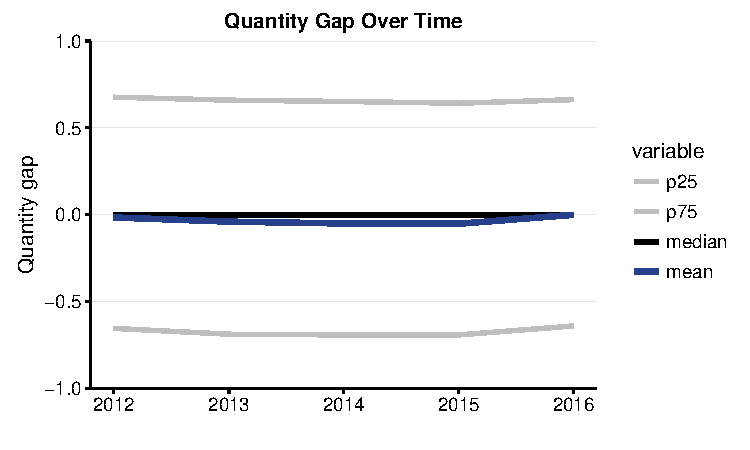
\includegraphics{Figs/quantity_time-1} \end{center}

\textbf{Quantity trade gap across products}

\begin{Shaded}
\begin{Highlighting}[]
\NormalTok{products <-}\StringTok{ }\NormalTok{hs12[, .(}\DataTypeTok{mean =} \KeywordTok{as.double}\NormalTok{(}\KeywordTok{mean}\NormalTok{(Qty_log_gap)),}
                     \DataTypeTok{median =} \KeywordTok{as.double}\NormalTok{(}\KeywordTok{median}\NormalTok{(Qty_log_gap)),}
                     \DataTypeTok{p25 =} \KeywordTok{as.double}\NormalTok{(}\KeywordTok{quantile}\NormalTok{(Qty_log_gap,.}\DecValTok{25}\NormalTok{)),}
                     \DataTypeTok{p75 =} \KeywordTok{as.double}\NormalTok{(}\KeywordTok{quantile}\NormalTok{(Qty_log_gap,.}\DecValTok{75}\NormalTok{))}
\NormalTok{),}
\NormalTok{by=}\StringTok{ `}\DataTypeTok{Commodity Code}\StringTok{`}\NormalTok{]}

\KeywordTok{ggplot}\NormalTok{(}\DataTypeTok{data=}\NormalTok{products, }\KeywordTok{aes}\NormalTok{(mean)) +}
\StringTok{  }\KeywordTok{geom_histogram}\NormalTok{(}\DataTypeTok{col=}\StringTok{"royalblue4"}\NormalTok{,}
                 \DataTypeTok{fill=}\StringTok{"royalblue4"}\NormalTok{,}
                 \DataTypeTok{alpha=}\NormalTok{.}\DecValTok{2}\NormalTok{) +}
\StringTok{  }\KeywordTok{background_grid}\NormalTok{(}\DataTypeTok{major =} \StringTok{'y'}\NormalTok{, }\DataTypeTok{minor =} \StringTok{"none"}\NormalTok{) +}
\StringTok{  }\KeywordTok{scale_y_continuous}\NormalTok{(}\DataTypeTok{expand =} \KeywordTok{c}\NormalTok{(}\DecValTok{0}\NormalTok{, }\DecValTok{0}\NormalTok{), }\DataTypeTok{limits =} \KeywordTok{c}\NormalTok{(}\DecValTok{0}\NormalTok{,}\DecValTok{300}\NormalTok{), }\DataTypeTok{minor_breaks =} \OtherTok{NULL}\NormalTok{) +}
\StringTok{  }\KeywordTok{labs}\NormalTok{(}\DataTypeTok{title=}\StringTok{"Mean Quantity Gap Across Products"}\NormalTok{) +}
\StringTok{  }\KeywordTok{labs}\NormalTok{(}\DataTypeTok{x=}\StringTok{"Quantity gap"}\NormalTok{, }\DataTypeTok{y=}\StringTok{"Number of products"}\NormalTok{)}
\end{Highlighting}
\end{Shaded}

\begin{center}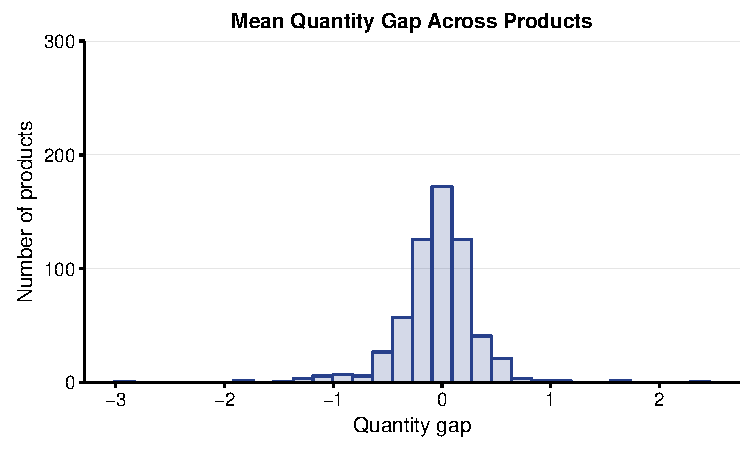
\includegraphics{Figs/quantity_products-1} \end{center}

\begin{Shaded}
\begin{Highlighting}[]
\KeywordTok{ggplot}\NormalTok{(}\DataTypeTok{data=}\NormalTok{products, }\KeywordTok{aes}\NormalTok{(median)) +}
\StringTok{  }\KeywordTok{geom_histogram}\NormalTok{(}\DataTypeTok{col=}\StringTok{"royalblue4"}\NormalTok{,}
                 \DataTypeTok{fill=}\StringTok{"royalblue4"}\NormalTok{,}
                 \DataTypeTok{alpha=}\NormalTok{.}\DecValTok{2}\NormalTok{) +}
\StringTok{  }\KeywordTok{background_grid}\NormalTok{(}\DataTypeTok{major =} \StringTok{'y'}\NormalTok{, }\DataTypeTok{minor =} \StringTok{"none"}\NormalTok{) +}
\StringTok{  }\KeywordTok{scale_y_continuous}\NormalTok{(}\DataTypeTok{expand =} \KeywordTok{c}\NormalTok{(}\DecValTok{0}\NormalTok{, }\DecValTok{0}\NormalTok{)) +}
\StringTok{  }\KeywordTok{labs}\NormalTok{(}\DataTypeTok{title=}\StringTok{"Median Quantity Gap Across Products"}\NormalTok{) +}
\StringTok{  }\KeywordTok{labs}\NormalTok{(}\DataTypeTok{x=}\StringTok{"Quantity gap"}\NormalTok{, }\DataTypeTok{y=}\StringTok{"Number of products"}\NormalTok{)}
\end{Highlighting}
\end{Shaded}

\begin{center}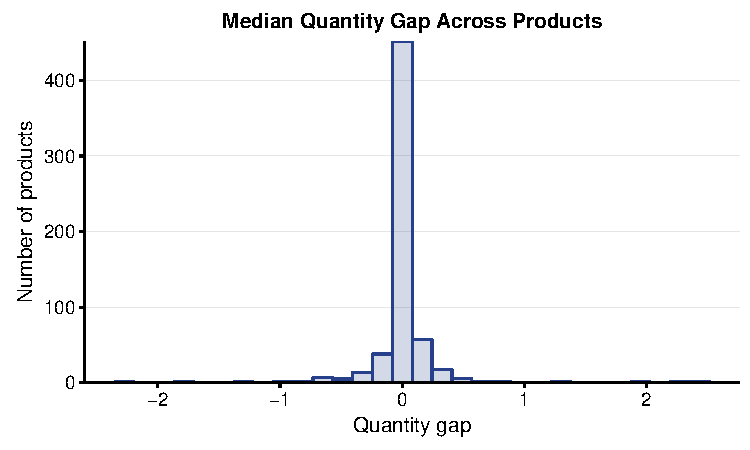
\includegraphics{Figs/quantity_products-2} \end{center}

\begin{Shaded}
\begin{Highlighting}[]
\KeywordTok{ggplot}\NormalTok{(}\DataTypeTok{data=}\NormalTok{products, }\KeywordTok{aes}\NormalTok{(p25)) +}
\StringTok{  }\KeywordTok{geom_histogram}\NormalTok{(}\DataTypeTok{col=}\StringTok{"royalblue4"}\NormalTok{,}
                 \DataTypeTok{fill=}\StringTok{"royalblue4"}\NormalTok{,}
                 \DataTypeTok{alpha=}\NormalTok{.}\DecValTok{2}\NormalTok{) +}
\StringTok{  }\KeywordTok{background_grid}\NormalTok{(}\DataTypeTok{major =} \StringTok{'y'}\NormalTok{, }\DataTypeTok{minor =} \StringTok{"none"}\NormalTok{) +}
\StringTok{  }\KeywordTok{scale_y_continuous}\NormalTok{(}\DataTypeTok{expand =} \KeywordTok{c}\NormalTok{(}\DecValTok{0}\NormalTok{, }\DecValTok{0}\NormalTok{), }\DataTypeTok{limits =} \KeywordTok{c}\NormalTok{(}\DecValTok{0}\NormalTok{,}\DecValTok{200}\NormalTok{), }\DataTypeTok{minor_breaks =} \OtherTok{NULL}\NormalTok{) +}
\StringTok{  }\KeywordTok{labs}\NormalTok{(}\DataTypeTok{title=}\StringTok{"25th Percentile Quantity Gap Across Products"}\NormalTok{) +}
\StringTok{  }\KeywordTok{labs}\NormalTok{(}\DataTypeTok{x=}\StringTok{"Trade gap"}\NormalTok{, }\DataTypeTok{y=}\StringTok{"Number of products"}\NormalTok{)}
\end{Highlighting}
\end{Shaded}

\begin{center}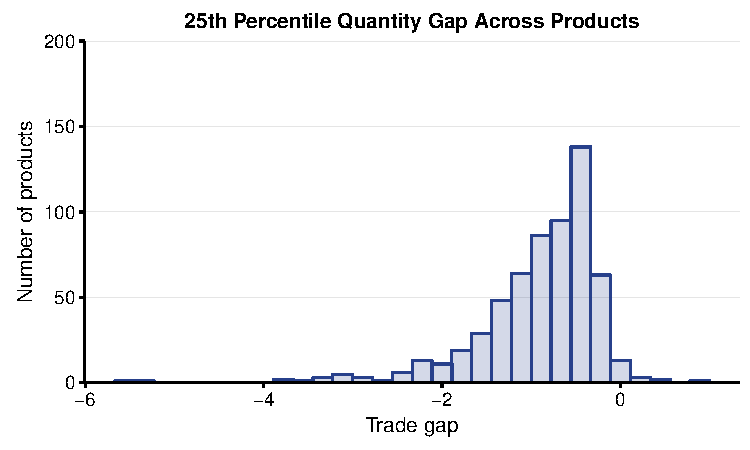
\includegraphics{Figs/quantity_products-3} \end{center}

\begin{Shaded}
\begin{Highlighting}[]
\KeywordTok{ggplot}\NormalTok{(}\DataTypeTok{data=}\NormalTok{products, }\KeywordTok{aes}\NormalTok{(p75)) +}
\StringTok{  }\KeywordTok{geom_histogram}\NormalTok{(}\DataTypeTok{col=}\StringTok{"royalblue4"}\NormalTok{,}
                 \DataTypeTok{fill=}\StringTok{"royalblue4"}\NormalTok{,}
                 \DataTypeTok{alpha=}\NormalTok{.}\DecValTok{2}\NormalTok{) +}
\StringTok{  }\KeywordTok{scale_y_continuous}\NormalTok{(}\DataTypeTok{expand =} \KeywordTok{c}\NormalTok{(}\DecValTok{0}\NormalTok{, }\DecValTok{0}\NormalTok{), }\DataTypeTok{limits =} \KeywordTok{c}\NormalTok{(}\DecValTok{0}\NormalTok{,}\DecValTok{200}\NormalTok{), }\DataTypeTok{minor_breaks =} \OtherTok{NULL}\NormalTok{) +}
\StringTok{  }\KeywordTok{background_grid}\NormalTok{(}\DataTypeTok{major =} \StringTok{'y'}\NormalTok{, }\DataTypeTok{minor =} \StringTok{"none"}\NormalTok{) +}
\StringTok{  }\KeywordTok{labs}\NormalTok{(}\DataTypeTok{title=}\StringTok{"75th Percentile Quantity Gap Across Products"}\NormalTok{) +}
\StringTok{  }\KeywordTok{labs}\NormalTok{(}\DataTypeTok{x=}\StringTok{"Trade gap"}\NormalTok{, }\DataTypeTok{y=}\StringTok{"Number of products"}\NormalTok{)}
\end{Highlighting}
\end{Shaded}

\begin{center}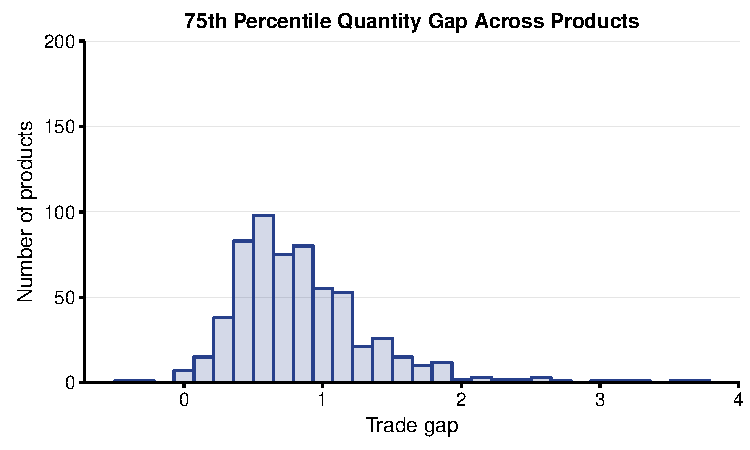
\includegraphics{Figs/quantity_products-4} \end{center}

\textbf{Quantity trade gap across country pairs}

\begin{Shaded}
\begin{Highlighting}[]
\NormalTok{countries <-}\StringTok{ }\NormalTok{hs12[, .(}\DataTypeTok{mean =} \KeywordTok{as.double}\NormalTok{(}\KeywordTok{mean}\NormalTok{(Qty_log_gap)),}
                      \DataTypeTok{median =} \KeywordTok{as.double}\NormalTok{(}\KeywordTok{median}\NormalTok{(Qty_log_gap)),}
                      \DataTypeTok{p25 =} \KeywordTok{as.double}\NormalTok{(}\KeywordTok{quantile}\NormalTok{(Qty_log_gap,.}\DecValTok{25}\NormalTok{)),}
                      \DataTypeTok{p75 =} \KeywordTok{as.double}\NormalTok{(}\KeywordTok{quantile}\NormalTok{(Qty_log_gap,.}\DecValTok{75}\NormalTok{))}
\NormalTok{),}
\NormalTok{by=}\StringTok{ }\KeywordTok{c}\NormalTok{(}\StringTok{"Importer"}\NormalTok{, }\StringTok{"Exporter"}\NormalTok{)]}

\KeywordTok{ggplot}\NormalTok{(}\DataTypeTok{data=}\NormalTok{countries, }\KeywordTok{aes}\NormalTok{(mean)) +}
\StringTok{  }\KeywordTok{geom_histogram}\NormalTok{(}\DataTypeTok{col=}\StringTok{"royalblue4"}\NormalTok{,}
                 \DataTypeTok{fill=}\StringTok{"royalblue4"}\NormalTok{,}
                 \DataTypeTok{alpha=}\NormalTok{.}\DecValTok{2}\NormalTok{) +}
\StringTok{  }\KeywordTok{background_grid}\NormalTok{(}\DataTypeTok{major =} \StringTok{'y'}\NormalTok{, }\DataTypeTok{minor =} \StringTok{"none"}\NormalTok{) +}
\StringTok{  }\KeywordTok{scale_y_continuous}\NormalTok{(}\DataTypeTok{expand =} \KeywordTok{c}\NormalTok{(}\DecValTok{0}\NormalTok{, }\DecValTok{0}\NormalTok{), }\DataTypeTok{limits =} \KeywordTok{c}\NormalTok{(}\DecValTok{0}\NormalTok{,}\DecValTok{2000}\NormalTok{), }\DataTypeTok{minor_breaks =} \OtherTok{NULL}\NormalTok{) +}
\StringTok{  }\KeywordTok{labs}\NormalTok{(}\DataTypeTok{title=}\StringTok{"Mean Quantity Gap Across Country Pairs"}\NormalTok{) +}
\StringTok{  }\KeywordTok{labs}\NormalTok{(}\DataTypeTok{x=}\StringTok{"Quantity gap"}\NormalTok{, }\DataTypeTok{y=}\StringTok{"Number of pairs"}\NormalTok{)}
\end{Highlighting}
\end{Shaded}

\begin{center}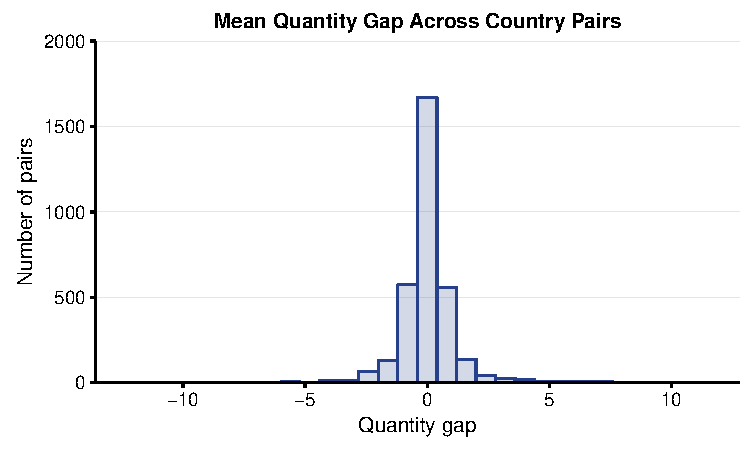
\includegraphics{Figs/quantity_pairs-1} \end{center}

\begin{Shaded}
\begin{Highlighting}[]
\KeywordTok{ggplot}\NormalTok{(}\DataTypeTok{data=}\NormalTok{countries, }\KeywordTok{aes}\NormalTok{(median)) +}
\StringTok{  }\KeywordTok{geom_histogram}\NormalTok{(}\DataTypeTok{col=}\StringTok{"royalblue4"}\NormalTok{,}
                 \DataTypeTok{fill=}\StringTok{"royalblue4"}\NormalTok{,}
                 \DataTypeTok{alpha=}\NormalTok{.}\DecValTok{2}\NormalTok{) +}
\StringTok{  }\KeywordTok{background_grid}\NormalTok{(}\DataTypeTok{major =} \StringTok{'y'}\NormalTok{, }\DataTypeTok{minor =} \StringTok{"none"}\NormalTok{) +}
\StringTok{  }\KeywordTok{scale_y_continuous}\NormalTok{(}\DataTypeTok{limits =} \KeywordTok{c}\NormalTok{(}\DecValTok{0}\NormalTok{,}\DecValTok{2500}\NormalTok{), }\DataTypeTok{minor_breaks =} \OtherTok{NULL}\NormalTok{) +}
\StringTok{  }\KeywordTok{labs}\NormalTok{(}\DataTypeTok{title=}\StringTok{"Median Quantity Gap Across Country Pairs"}\NormalTok{) +}
\StringTok{  }\KeywordTok{labs}\NormalTok{(}\DataTypeTok{x=}\StringTok{"Quantity gap"}\NormalTok{, }\DataTypeTok{y=}\StringTok{"Number of pairs"}\NormalTok{)}
\end{Highlighting}
\end{Shaded}

\begin{center}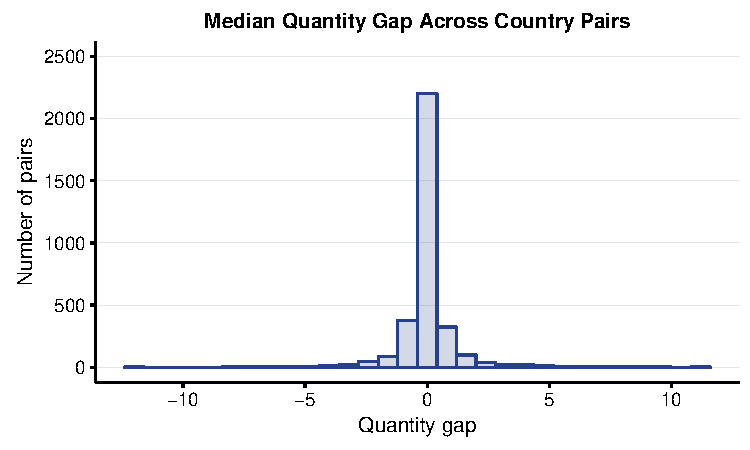
\includegraphics{Figs/quantity_pairs-2} \end{center}

\begin{Shaded}
\begin{Highlighting}[]
\KeywordTok{ggplot}\NormalTok{(}\DataTypeTok{data=}\NormalTok{countries, }\KeywordTok{aes}\NormalTok{(p25)) +}
\StringTok{  }\KeywordTok{geom_histogram}\NormalTok{(}\DataTypeTok{col=}\StringTok{"royalblue4"}\NormalTok{,}
                 \DataTypeTok{fill=}\StringTok{"royalblue4"}\NormalTok{,}
                 \DataTypeTok{alpha=}\NormalTok{.}\DecValTok{2}\NormalTok{) +}
\StringTok{  }\KeywordTok{background_grid}\NormalTok{(}\DataTypeTok{major =} \StringTok{'y'}\NormalTok{, }\DataTypeTok{minor =} \StringTok{"none"}\NormalTok{) +}
\StringTok{  }\KeywordTok{scale_y_continuous}\NormalTok{(}\DataTypeTok{expand =} \KeywordTok{c}\NormalTok{(}\DecValTok{0}\NormalTok{, }\DecValTok{0}\NormalTok{), }\DataTypeTok{limits =} \KeywordTok{c}\NormalTok{(}\DecValTok{0}\NormalTok{,}\DecValTok{1500}\NormalTok{), }\DataTypeTok{minor_breaks =} \OtherTok{NULL}\NormalTok{) +}
\StringTok{  }\KeywordTok{labs}\NormalTok{(}\DataTypeTok{title=}\StringTok{"25th Percentile Quantity Gap Across Country Pairs"}\NormalTok{) +}
\StringTok{  }\KeywordTok{labs}\NormalTok{(}\DataTypeTok{x=}\StringTok{"Quantity gap"}\NormalTok{, }\DataTypeTok{y=}\StringTok{"Number of pairs"}\NormalTok{)}
\end{Highlighting}
\end{Shaded}

\begin{center}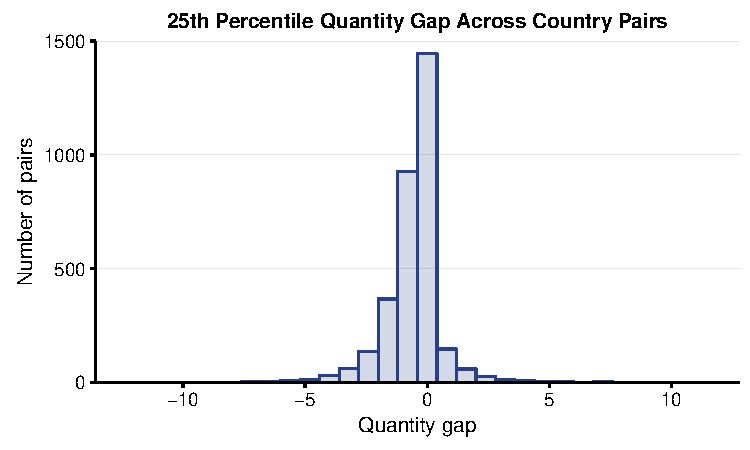
\includegraphics{Figs/quantity_pairs-3} \end{center}

\begin{Shaded}
\begin{Highlighting}[]
\KeywordTok{ggplot}\NormalTok{(}\DataTypeTok{data=}\NormalTok{countries, }\KeywordTok{aes}\NormalTok{(p75)) +}
\StringTok{  }\KeywordTok{geom_histogram}\NormalTok{(}\DataTypeTok{col=}\StringTok{"royalblue4"}\NormalTok{,}
                 \DataTypeTok{fill=}\StringTok{"royalblue4"}\NormalTok{,}
                 \DataTypeTok{alpha=}\NormalTok{.}\DecValTok{2}\NormalTok{) +}
\StringTok{  }\KeywordTok{background_grid}\NormalTok{(}\DataTypeTok{major =} \StringTok{'y'}\NormalTok{, }\DataTypeTok{minor =} \StringTok{"none"}\NormalTok{) +}
\StringTok{  }\KeywordTok{scale_y_continuous}\NormalTok{(}\DataTypeTok{expand =} \KeywordTok{c}\NormalTok{(}\DecValTok{0}\NormalTok{, }\DecValTok{0}\NormalTok{), }\DataTypeTok{limits =} \KeywordTok{c}\NormalTok{(}\DecValTok{0}\NormalTok{,}\DecValTok{2000}\NormalTok{), }\DataTypeTok{minor_breaks =} \OtherTok{NULL}\NormalTok{) +}
\StringTok{  }\KeywordTok{labs}\NormalTok{(}\DataTypeTok{title=}\StringTok{"75th Percentile Quantity Gap Across Country Pairs"}\NormalTok{) +}
\StringTok{  }\KeywordTok{labs}\NormalTok{(}\DataTypeTok{x=}\StringTok{"Quantity gap"}\NormalTok{, }\DataTypeTok{y=}\StringTok{"Number of pairs"}\NormalTok{)}
\end{Highlighting}
\end{Shaded}

\begin{center}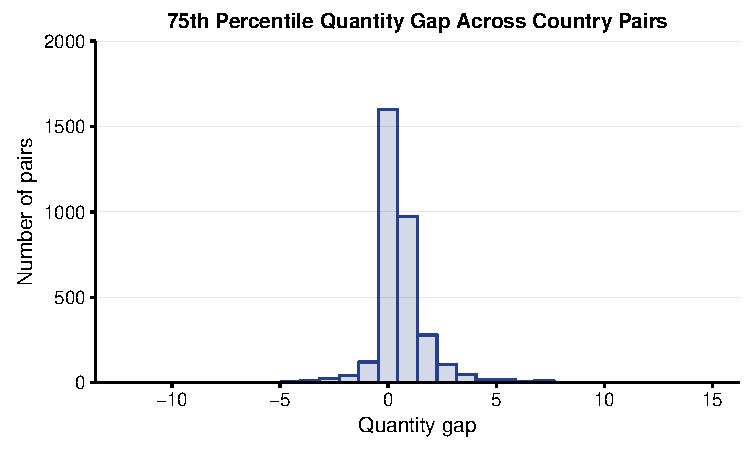
\includegraphics{Figs/quantity_pairs-4} \end{center}

\begin{Shaded}
\begin{Highlighting}[]
\KeywordTok{rm}\NormalTok{(periods, products, countries)}
\end{Highlighting}
\end{Shaded}

\textbf{Quantity year coefficients controlling for product codes and
country pairs}

\begin{Shaded}
\begin{Highlighting}[]
\NormalTok{hs12$Period <-}\StringTok{ }\KeywordTok{as.Date}\NormalTok{(hs12$Period, }\StringTok{"%Y"}\NormalTok{)}
\NormalTok{hs12$Period <-}\StringTok{ }\KeywordTok{floor_date}\NormalTok{(hs12$Period,}\StringTok{"year"}\NormalTok{)}

\NormalTok{hs12$Period.f <-}\StringTok{ }\KeywordTok{factor}\NormalTok{(hs12$Period)}
\NormalTok{hs12$Products.f <-}\StringTok{ }\KeywordTok{factor}\NormalTok{(hs12$}\StringTok{`}\DataTypeTok{Commodity Code}\StringTok{`}\NormalTok{)}

\NormalTok{hs12$Importer.f <-}\StringTok{ }\KeywordTok{factor}\NormalTok{(hs12$}\StringTok{`}\DataTypeTok{Reporter Code}\StringTok{`}\NormalTok{)}
\NormalTok{hs12$Exporter.f <-}\StringTok{ }\KeywordTok{factor}\NormalTok{(hs12$}\StringTok{`}\DataTypeTok{Partner Code}\StringTok{`}\NormalTok{)}
\NormalTok{hs12$Pairs.f <-}\StringTok{ }\KeywordTok{with}\NormalTok{(hs12, }\KeywordTok{interaction}\NormalTok{(Importer.f, Exporter.f))}

\NormalTok{reg <-}\StringTok{ }\KeywordTok{felm}\NormalTok{(Qty_log_gap ~}\StringTok{ }\DecValTok{1} \NormalTok{|}\StringTok{ }\NormalTok{Period.f +}\StringTok{ }\NormalTok{Products.f +}\StringTok{ }\NormalTok{Pairs.f,}
            \DataTypeTok{data =} \NormalTok{hs12,}
            \DataTypeTok{exactDOF =} \OtherTok{FALSE}\NormalTok{,}
            \DataTypeTok{keepX =} \OtherTok{FALSE}\NormalTok{,}
            \DataTypeTok{keepCX =} \OtherTok{FALSE}\NormalTok{)}

\NormalTok{fes <-}\StringTok{ }\KeywordTok{getfe}\NormalTok{(reg,}
             \DataTypeTok{se=}\OtherTok{TRUE}\NormalTok{,}
             \DataTypeTok{bN =} \DecValTok{50}
\NormalTok{)}

\NormalTok{periodfes <-}\StringTok{ }\KeywordTok{subset}\NormalTok{(fes,fe ==}\StringTok{ "Period.f"}\NormalTok{)}

\NormalTok{periodfes$ci_ub <-}\StringTok{ }\NormalTok{periodfes$effect +}\StringTok{ }\NormalTok{(}\FloatTok{1.96} \NormalTok{*}\StringTok{ }\NormalTok{periodfes$se)}
\NormalTok{periodfes$ci_lb <-}\StringTok{ }\NormalTok{periodfes$effect -}\StringTok{ }\NormalTok{(}\FloatTok{1.96} \NormalTok{*}\StringTok{ }\NormalTok{periodfes$se)}
\NormalTok{periodfes <-}\StringTok{ }\KeywordTok{merge}\NormalTok{(periodfes,}\KeywordTok{unique}\NormalTok{(hs12[,}\KeywordTok{list}\NormalTok{(Period,Period.f)]),}\DataTypeTok{by.x =} \StringTok{"idx"}\NormalTok{,}\DataTypeTok{by.y=}\StringTok{"Period.f"}\NormalTok{)}
\NormalTok{periodfes <-}\StringTok{ }\KeywordTok{rename}\NormalTok{(periodfes, }\DataTypeTok{period =} \NormalTok{Period)}

\KeywordTok{ggplot}\NormalTok{(}\DataTypeTok{data =} \NormalTok{periodfes, }\KeywordTok{aes}\NormalTok{(period,effect)) +}
\StringTok{  }\KeywordTok{geom_errorbar}\NormalTok{(}\KeywordTok{aes}\NormalTok{(}\DataTypeTok{ymin =} \NormalTok{ci_lb, }\DataTypeTok{ymax =} \NormalTok{ci_ub), }\DataTypeTok{color =} \StringTok{"grey35"}\NormalTok{) +}
\StringTok{  }\KeywordTok{geom_line}\NormalTok{(}\DataTypeTok{color =} \StringTok{"royalblue4"}\NormalTok{, }\DataTypeTok{size =} \DecValTok{1}\NormalTok{) +}
\StringTok{  }\KeywordTok{geom_point}\NormalTok{(}\DataTypeTok{color =} \StringTok{"royalblue4"}\NormalTok{) +}
\StringTok{  }\KeywordTok{background_grid}\NormalTok{(}\DataTypeTok{major =} \StringTok{'y'}\NormalTok{, }\DataTypeTok{minor =} \StringTok{"none"}\NormalTok{) +}
\StringTok{  }\KeywordTok{scale_y_continuous}\NormalTok{(}\DataTypeTok{expand =} \KeywordTok{c}\NormalTok{(}\DecValTok{0}\NormalTok{, }\DecValTok{0}\NormalTok{), }\DataTypeTok{limits =} \KeywordTok{c}\NormalTok{(-.}\DecValTok{05}\NormalTok{, .}\DecValTok{10}\NormalTok{), }\DataTypeTok{breaks=}\KeywordTok{seq}\NormalTok{(-.}\DecValTok{05}\NormalTok{, .}\DecValTok{10}\NormalTok{, .}\DecValTok{05}\NormalTok{)) +}
\StringTok{  }\KeywordTok{xlab}\NormalTok{(}\DataTypeTok{label =} \StringTok{""}\NormalTok{) +}
\StringTok{  }\KeywordTok{ylab}\NormalTok{(}\DataTypeTok{label =} \StringTok{"Quantity gap"}\NormalTok{) +}
\StringTok{  }\KeywordTok{labs}\NormalTok{(}\DataTypeTok{title =} \StringTok{"Quantity Gap Over Time, Controlling for Product/Country Pair"}\NormalTok{)}
\end{Highlighting}
\end{Shaded}

\begin{center}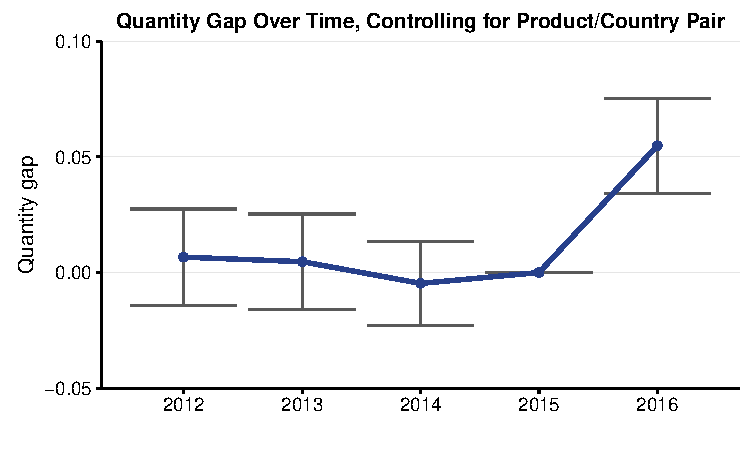
\includegraphics{Figs/quantity_years_reg-1} \end{center}

\textbf{Quantity product code coefficients controlling for country pairs
and years}

\begin{Shaded}
\begin{Highlighting}[]
\NormalTok{productfes <-}\StringTok{ }\KeywordTok{subset}\NormalTok{(fes,fe ==}\StringTok{ "Products.f"}\NormalTok{)}
\NormalTok{productfes <-}\StringTok{ }\NormalTok{productfes[,}\KeywordTok{c}\NormalTok{(}\StringTok{"effect"}\NormalTok{,}\StringTok{"idx"}\NormalTok{)]}

\KeywordTok{ggplot}\NormalTok{(}\DataTypeTok{data=}\NormalTok{productfes, }\KeywordTok{aes}\NormalTok{(effect)) +}
\StringTok{  }\KeywordTok{geom_histogram}\NormalTok{(}\DataTypeTok{col=}\StringTok{"royalblue4"}\NormalTok{,}
                 \DataTypeTok{fill=}\StringTok{"royalblue4"}\NormalTok{,}
                 \DataTypeTok{alpha=}\NormalTok{.}\DecValTok{2}\NormalTok{) +}
\StringTok{  }\KeywordTok{background_grid}\NormalTok{(}\DataTypeTok{major =} \StringTok{'y'}\NormalTok{, }\DataTypeTok{minor =} \StringTok{"none"}\NormalTok{) +}
\StringTok{  }\KeywordTok{scale_y_continuous}\NormalTok{(}\DataTypeTok{expand =} \KeywordTok{c}\NormalTok{(}\DecValTok{0}\NormalTok{, }\DecValTok{0}\NormalTok{), }\DataTypeTok{limits =} \KeywordTok{c}\NormalTok{(}\DecValTok{0}\NormalTok{,}\DecValTok{300}\NormalTok{), }\DataTypeTok{minor_breaks =} \OtherTok{NULL}\NormalTok{) +}
\StringTok{  }\KeywordTok{labs}\NormalTok{(}\DataTypeTok{title=}\StringTok{"Quantity Gap Across Products, Controlling for Country Pair/Year"}\NormalTok{) +}
\StringTok{  }\KeywordTok{labs}\NormalTok{(}\DataTypeTok{x=}\StringTok{"Quantity gap"}\NormalTok{, }\DataTypeTok{y=}\StringTok{"Number of Products"}\NormalTok{)}
\end{Highlighting}
\end{Shaded}

\begin{center}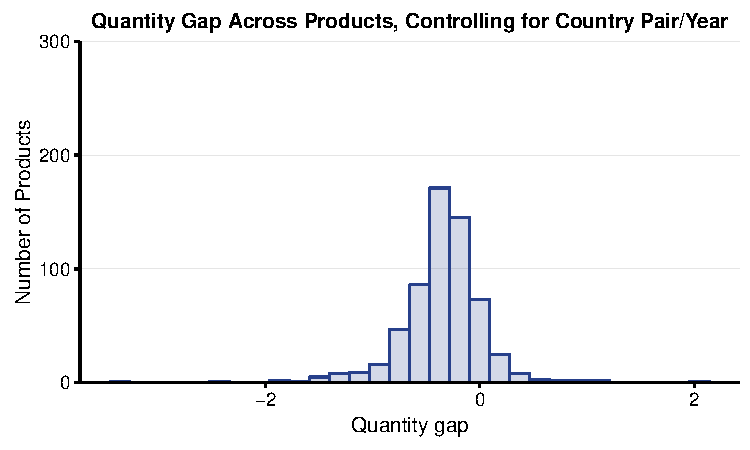
\includegraphics{Figs/quantity_products_reg-1} \end{center}

\textbf{Quantity country pair coefficients controlling for years and
product codes}

\begin{Shaded}
\begin{Highlighting}[]
\NormalTok{pairfes <-}\StringTok{ }\KeywordTok{subset}\NormalTok{(fes,fe ==}\StringTok{ "Pairs.f"}\NormalTok{)}
\NormalTok{pairfes <-}\StringTok{ }\NormalTok{pairfes[,}\KeywordTok{c}\NormalTok{(}\StringTok{"effect"}\NormalTok{,}\StringTok{"idx"}\NormalTok{)]}

\KeywordTok{ggplot}\NormalTok{(}\DataTypeTok{data=}\NormalTok{pairfes, }\KeywordTok{aes}\NormalTok{(effect)) +}
\StringTok{  }\KeywordTok{geom_histogram}\NormalTok{(}\DataTypeTok{col=}\StringTok{"royalblue4"}\NormalTok{,}
                 \DataTypeTok{fill=}\StringTok{"royalblue4"}\NormalTok{,}
                 \DataTypeTok{alpha=}\NormalTok{.}\DecValTok{2}\NormalTok{) +}
\StringTok{  }\KeywordTok{background_grid}\NormalTok{(}\DataTypeTok{major =} \StringTok{'y'}\NormalTok{, }\DataTypeTok{minor =} \StringTok{"none"}\NormalTok{) +}
\StringTok{  }\KeywordTok{scale_y_continuous}\NormalTok{(}\DataTypeTok{expand =} \KeywordTok{c}\NormalTok{(}\DecValTok{0}\NormalTok{, }\DecValTok{0}\NormalTok{), }\DataTypeTok{limits =} \KeywordTok{c}\NormalTok{(}\DecValTok{0}\NormalTok{,}\DecValTok{1500}\NormalTok{), }\DataTypeTok{minor_breaks =} \OtherTok{NULL}\NormalTok{) +}
\StringTok{  }\KeywordTok{labs}\NormalTok{(}\DataTypeTok{title=}\StringTok{"Quantity Gap Across Country Pairs, Controlling for Product/Year"}\NormalTok{) +}
\StringTok{  }\KeywordTok{labs}\NormalTok{(}\DataTypeTok{x=}\StringTok{"Quantity gap"}\NormalTok{, }\DataTypeTok{y=}\StringTok{"Number of country pairs"}\NormalTok{)}
\end{Highlighting}
\end{Shaded}

\begin{center}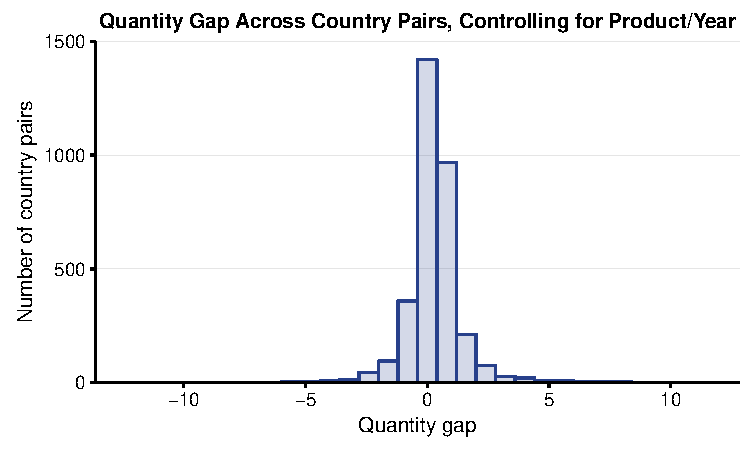
\includegraphics{Figs/quantity_pairs_reg-1} \end{center}

\begin{Shaded}
\begin{Highlighting}[]
\KeywordTok{rm}\NormalTok{(fes, hs12, pairfes, periodfes, productfes, reg)}
\end{Highlighting}
\end{Shaded}


\end{document}
